\documentclass[11pt,letterpaper]{article}

\usepackage{showlabels}
\usepackage{fullpage}
\usepackage{pslatex}
\usepackage[english]{babel}
\usepackage[utf8]{inputenc}
\usepackage{amsmath}
\usepackage{bm}
\usepackage{xcolor}
\usepackage{url}
\usepackage{rotating}
\usepackage{natbib}
\usepackage{amssymb}
\usepackage{lingmacros}


%\usepackage{linguex}
%\usepackage{lingmacros}

\usepackage{CJKutf8}
\newcommand{\korean}[1]{\begin{CJK}{UTF8}{mj}#1\end{CJK}}

\usepackage{tikz}


\usepackage{colortbl}

%\usepackage{xeCJK}

\usepackage{natbib}
\bibliographystyle{unsrtnat}

%\usepackage{latexsym}
\usepackage[english]{babel}
\usepackage[utf8]{inputenc}
\usepackage{bm}
\usepackage{graphicx}
%\usepackage{tikz}
\usepackage{xcolor}
\usepackage{url}
%\usepackage[colorinlistoftodos]{todonotes}
\usepackage{rotating}
\usepackage{multirow}




\usepackage{hyperref}

\usepackage{tikz-dependency}
\usepackage{changepage}
\usepackage{longtable}


\newcommand{\R}[0]{\mathbb{R}}
\newcommand{\Prob}[0]{\mathbb{P}}
\newcommand{\Ff}[0]{\mathcal{F}}

\usepackage{multirow}

\newcommand{\soft}[1]{}
\newcommand{\nopreview}[1]{}
\newcommand\comment[1]{{\color{red}#1}}
\newcommand\michael[1]{{\color{red}(#1)}}
\newcommand\mhahn[1]{{\color{red}(#1)}}
\newcommand\becky[1]{{\color{blue}(#1)}}
\newcommand\note[1]{{\color{red}(#1)}}
\newcommand\jd[1]{{\color{red}(#1)}}
\newcommand\rljf[1]{{\color{red}(#1)}}
\newcommand{\key}[1]{\textbf{#1}}

\DeclareMathOperator*{\argmax}{arg\,max}
\DeclareMathOperator*{\argmin}{arg\,min}
\DeclareMathOperator{\E}{\mathop{\mathbb{E}}}



%\usepackage{lingmacros}
%\usepackage{linguex}


\usepackage{amsthm}

\newcommand{\thetad}[0]{{\theta-d}}
\newcommand{\thetal}[0]{{\theta-{LM}}}

\newcounter{theorem}
\newtheorem{proposition}[theorem]{Proposition}
\newtheorem{thm}[theorem]{Theorem}
\newtheorem{corollary}[theorem]{Corollary}
\newtheorem{question}[theorem]{Question}
\newtheorem{example}[theorem]{Example}
\newtheorem{defin}[theorem]{Definition}
\newtheorem{definition}[theorem]{Definition}
\newtheorem{lemma}[theorem]{Lemma}


%\usepackage{linguex}
%\newcommand{\key}[1]{\textbf{#1}}



\renewcommand{\thefigure}{S\arabic{figure}}
\renewcommand{\thetable}{S\arabic{table}}
\renewcommand{\thesection}{S\arabic{section}}

\newcommand{\utterance}{\mathcal{U}}
\newcommand{\tree}{\mathcal{T}}



\usepackage{siunitx}



\usepackage{longtable}



\frenchspacing
%\def\baselinestretch{0.975}

%\emnlpfinalcopy
%\def\emnlppaperid{496}

\title{Morpheme Ordering across Languages reflects optimization for Memory Efficiency}

\begin{document}

\maketitle

\begin{abstract}
The order of morphemes in a word shows well-documented tendencies across languages.
Previous work has explained these in terms of notions such as semantic scope and relevance.
A recent theory argues that word and morpheme order in language optimizes a tradeoff between Memory and surprisal, and provided initial evidence from two languages that morpheme order can partly be explained by optimization for this treadeoff.
In this work, we test this idea more extensively using data from four additional agglutinative languages with significant amounts of morphology, in both verb and noun inflection.
We find that the memory-surprisal tradeoff predicts order in most cases with high accuracy.
We also find that it accounts for several, previously documented, universal properties, such as the relative order of number and case suffixes on nouns.
Our work adds to a growing body of work suggesting that many properties of language arise from cognitive principles.
\end{abstract}


\section{Introduction}

Human language encodes thoughts into linear strings of words, and ultimately sounds.
Across languages, words are composed of morphemes, commonly defined as the smallest meaning-bearing units of language  (CITE).
%In many cases, words can be segmented into a sequence of morphemes, as in
For instance, the English word ``runners'' can be decomposed into three morphemes: the root run- indicating an action, the suffix -er- indicating someone performing an action, and plural -s indicating a group of several referents.
The order of morphemes within a word follows well-documented cross-linguistic tendencies, for instance, morphemes deriving new words (e.g., English -er deriving nouns from verbs) are ordered closer to the root than inflectional morphemes (e.g., English plural -s).
Another well-documented universal applying to languages with richer morphology is Greenbergs' Universal X:
Plural markers tend to be closer to noun stems than case markers \citep[112]{greenberg1963universals} (TODO example from some language).
In morphologically rich languages, verbs often have a string of two or more affix morphemes attached to a root, and the typological literature has documented universal tendencies, such as a preference for morphemes changing the number of arguments to appear close to the root, while morphemes indicating agreement with subjects appear far away from the root \citep{bybee-morphology-1985}.

Explaining these linguistic universals has been an important subject of study.
Explanations have been stated in terms of the relative scope of different morphemes  \citep{rice2000morpheme}, parallelism between morphology and syntax \citep{givon1971historical,venneman1973explanation,baker1985the}, and the strength of their semantic association between different morphemes \citep{bybee-morphology-1985}.
%One family of explanations holds that those affixes are closest to the root that are most relevant to the root \citep{bybee-morphology-1985}.
%Other explanations suggest that morphemes are ordered based on (TODO CITE).

A recent theory proposes a cognitive explanation for word and morpheme order in language, arguing that ordering universals in language optimize processing effort under memory limitations \citep{Hahn2020modeling}.
Formally, they introduced the notion of a memory-surprisal tradeoff: Depending on how many memory resources a comprehender invests, they can achieve different levels of surprisal.
\citep{Hahn2020modeling} argue that order of words and morphemes in language optimizes this tradeoff.
Optimizing the memory-surprisal tradeoff amounts to putting elements together when they predict each other strongly, as measured by mutual information.
In a case study, \citep{Hahn2020modeling} apply this to morpheme ordering in verbs in two languages (Japanese and Sesotho), finding that optimization could partly reproduce morpheme ordering in these languages.
They also suggested that mutual information formalizes previous notions of strength of semantic association between morphemes \citep{bybee-morphology-1985}. %, such as \cite{bybee-morphology-1985}'s notion of \textit{relevance}.






In this work, we examine this theory on a broader basis.
First, we consider data from four additional languages, testing whether it accounts for universals of verb affix order documented by \cite{bybee-morphology-1985}.
Second, we consider nouns in addition to verbs, testing whether it accounts for Greenberg's Universal X.

We focus on languages with rich morphology where words tend to have multiple morphemes and these are mostly realized separately.
Such languages are referred to as agglutinative \cite{humboldt1836uber,greenberg1960a}.
We obtained data from four languages where substantial amounts of corpus data with detailed morphological annotation are available (Korean, Turkish, Hungarian, Finnish).
These languages have very substantial verbal inflection, and three of these languages (Turkish, Hungarian, Finnish) also have substantial noun inflection.
%Whereas \cite{Hahn2020modeling} only considered verb inflection, we also consider noun inflection across three languages.

% interesting https://www.eva.mpg.de/fileadmin/content_files/staff/haspelmt/pdf/Agglutination.pdf

%Greenberg 1963:  "the expression of number almost always comes between the noun base and the expression of case" (Greenberg 1963:112)

%Scope, Syntax, History
%Another family of explanations holds that morpheme ordering is to be explained diachronically, and that morpheme order reflects the order of independent words in earlier stages of a language.
%- Relevance, Proximity Principle, Iconicity




%Bybee on explanation:
%- regarding the historical explanation (Givon 1971, Vennemann 1973):
%Morphology is not always fossilizes syntax (Bybee and Brewer 1980, Bybee 1985 p. 39--40)


\section{Locality and the Memory--Surprisal Tradeoff}

A long line of work in linguistics has proposed principles of locality to account for word order regularities within and across languages.
An early example is \citep{behaghel1932deutsche}, who argued that elements that are closer together in meaning are closer together in form.
In word order, the Head Proximity principle of \citep{rijkhoff-word-1986} states that words are close to their syntactic heads, and this generalization has since found strong empirical support from data in many languages~\cite[e.g.][]{liu2008dependency, futrell-large-scale-2015-1, liu-dependency-2017}.
In morpheme ordering, \citep{bybee-morphology-1985} argues that morphemes are closer to the root when they are more relevant to it.
One explanation of such principles is in terms of iconicity in form-meaning correspondence \citep{givon1985iconicity}.
More recently, locality principles have been explained in terms of memory and efficiency in online processing \citep{hawkins-efficiency-2003}.
Based on considerations of memory limitations, \citet{futrell-noisy-context-2017} derived an information-theoretic locality principle that states that words are close to each other when they are highly predictive of each other (see also \citet{culbertson2020from}).
%This principle of information locality TODO


\citet{Hahn2020modeling} proposed a cognitive principle that aims to unify and formalize these locality principles in the form of a Memory--Surprisal Tradoff.
This is a cognitive account of the order of words and morphemes in human language, based on a formalization of memory efficiency in incremental processing.
The memory-surprisal tradeoff links information-theoretic models of memory limitations with surprisal theory.

Surprisal theory \citep{hale2001probabilistic, levy2008expectation} is a theory of the word-by-word processing difficulty in online processing.
It states that the processing effort on a word $w_t$ in context $w-1 ... w_{t-1}$ is proportional to its surprisal
     \begin{equation}   \label{eq:true-surp}
    \text{Difficulty} \propto -\log P(w_t | w_1\dots w_{t-1}).
\end{equation}
Surprisal as estimated by corpus-based methods or cloze is a successful predictor of reading time on naturalistic text \citep{smith2013effect,goodkind-predictive-2018,frank2019interaction,aurnhammer2019evaluating,wilcox2020predictive}. % (TODO citation based on Cloze).
Surprisal theory is a computational-level theory; it can be justified in terms of different mechanisms such as preactivation and integration~\citep{kuperberg2016we}.
\citet{Hahn2020modeling} argue that, due to limitations in human memory, human expectations in reality do not reflect the true context $w_1\dots w_{t-1}$, but some potentially lossy memory representation $m_t$ of the context $w_1\dots w_{t-1}$:
\begin{equation}   \label{eq:lossy-surp}
    \text{Difficulty} \propto -\log P(w_t | m_t).
\end{equation}
\citet{Hahn2020modeling} note that there is a tradeoff between average surprisal and memory capacity:
The more information a listener stores in $m_t$, the lower their surprisal will be on average.
This is because higher precision of memory leads to more precise expectations, which will achiever lower surprisal on average.

More formally, they consider functions $M$ describing how comprehenders update memory representations $m_{t-1}$ when observing a word (or morpheme) $w_t$ to a new memory state $m_t := M(m_{t-1}, w_t)$.
The memory capacity is formalized as the aveage number of bits required to encode $m_t$, i.e., its entropy:
\begin{equation*}
    \operatorname{H}[m_t] := - \sum_m P(m_t = m) \log_2 P(m_t=m)
\end{equation*}
where $m$ runs over possible memory states.
\citet{Hahn2020modeling} prove that there is a tradeoff between, on the one hand, the average surprisal $S\_M$, obtained by averaging $- \log P(w_t , m_t)$ across the words in a text, and the memory capacity $\operatorname{H}[m_t]$.

\mhahn{at this point illustrate with a figure?}

Based on this notion, \citet{Hahn2020modeling} proposed the Efficient Tradeoff Hypothesis, suggesting that human language orders elements in such a way that the memory-surprisal tradeoff curve has a particularly steep fall-off, compared to other possible orderings.


\citet{Hahn2020modeling} provide a method for estimating a bound on the memory-surprisal tradeoff from corpus data, and show that orderings achieve efficient tradeoffs when elements that predict each other are close together.
This method is based on the notion of mutual information, which quantifies the amount of statistical association between two random variables.
If $X, Z, Y$ are random variables, then the mutual information of $X$ and $Y$, conditioned on $Z$, is defined to be:
\begin{align}
\label{eq:mi}
    \operatorname{I}[X:Y,Z] &\equiv \sum_{x,y,z} P(x,y,z) \log \frac{P(x,y,z)}{P(x,z)P(y,z)}. % \text{ bits} \\
    %\nonumber
    %&= \operatorname{H}[X,Z] - \operatorname{H}[X,Y,Z] \\
    %\nonumber
    %&= \operatorname{H}[Y,Z] - \operatorname{H}[Y,X,Z].
\end{align}
The key quantity derived from this is the mutual information between elements (such as morphemes) that are some distance $t$, conditioned on the intervening elements:
\begin{equation*}
    I_t \equiv \operatorname{I}[w_t : w_0 , w_1, \dots, w_{t-1}].
\end{equation*}
Based on this notion, \citet{Hahn2020modeling}  prove the following bound on the memory-surprisal tradeoff :
\begin{thm}\label{prop:suboptimal}(Information locality bound, \citet{Hahn2020modeling})
For any positive integer $T$, let $M$ be a memory encoding function such that
\begin{equation}
\label{eq:memory-bound}
\operatorname{H}[m_t] \le \sum_{t=1}^T t I_t.
\end{equation}
Then we have a lower bound on the average surprisal $S_M$ under the memory encoding function $M$:
\begin{equation}
\label{eq:surprisal-bound}
S_M \ge S_\infty + \sum_{t=T+1}^\infty I_t.
\end{equation}
where $S_\infty$ is the average surprisal that would be achieved with perfectly veridical memory representations.
\end{thm}

\mhahn{again, at this point illustrate with a figure?}

A key consequence of this theorem is an information-theoretic notion of locality called Information locality:
Informally, orderings optimize this tradeoff when elements with high mutual information are closer together.
%Previously, a similar notion of information locality was derived by \citet{futrell2020lossy} for a specific family of memory representations $M$.
Information locality has had success as a predictor of word order \citep{futrell2019information}, in particular for universals of the order inside noun phrases \citep{culbertson2020from,hahn-information-theoretic-2018,DBLP:conf/acl/FutrellDS20}.



\citet{Hahn2020modeling} argue that information locality derives a range of locality principles proposed in the linguistic literature.
They provide evidence that it predicts closeness of syntactically related words.
They also provide preliminary evidence that it accounts for some properties of morpheme ordering and formalizes \cite{bybee-morphology-1985}'s idea that morphemes are closer together when they are more relevant to each other, using data of verb inflection in two languages (Japanese and Sesotho).

In this work, we aim to test the Memory-Surprisal Tradeoff as a predictor of morpheme ordering more broadly, using data from more languages and from different parts of speech.



\section{Morpheme Ordering and Ordering Universals}

In this section, we introduce some general crosslinguistic tendencies in morpheme ordering, including discussion of the the six languages, and the language universals that we seek to explain.

Languages apply inflection to different classes of words, including both open word classes such as nouns, verbs, and adjectives, and closed word classes, in particular pronouns.
In this work, we focus on open word classes, as these have productive paradigms that apply to thousands of words in a language, including words that newly enter the language, whereas pronominal inflection is restricted to a small number of words, often with idiosynractic and fossilized paradigms inherited from earlier stages of a language (CITE).
Among open word classes, inflection commonly applies to verbs, nouns, and adjectives (CITE).
We focus on nouns and verbs.
When adjectives are inflected, they often pattern with either verbs -- when they are used as predicates -- or nouns -- when they are used as attributes or independent nouns.

Nouns very commonly mark number and case morphologically.
%Number marking typically distinguishes singular and plural (person -- person-s).
%Case marking 
In some languages, possession is also marked on the noun (CITE).
Figure~\ref{fig:noun-inflection} shows fully inflected nouns in three languages from our sample, with endings for number, case, and possessor.
Number and case marking are the subject of a well-documented universal, namely \citep{greenberg1963universals}'s Universal 39:

\begin{adjustwidth}{6em}{6em}
\textsc{Greenberg's Universal 39}:
``the expression of number almost always comes between the noun base and the expression of case'' (Greenberg 1963:112).
\end{adjustwidth}
%It states that number affixes are closer to the stem than case affixes, if they appear on the same side.

This universal is supported by the example in Figure~\ref{fig:noun-inflection}.

%\ex.\ag. mi  rare mash yoo \\
%%Stem (3) (5) (8) \\
%see  \textsc{passive}  \textsc{politeness}  \textsc{future} \\
%`will be seen'
%\bg. mi taku nakat ta \\
%%Stem (6) (7) (8) \\
%see \textsc{desiderative} \textsc{negation} \textsc{past} \\
%`did not wish to see'


\begin{figure}
\begin{tabular}{lllllllll}
\textit{juttu-i-hi-si} \\
Stem-Plural-Illative-2SgPoss \\
`into your stories' (Finnish)
\end{tabular}
\begin{tabular}{lllllllll}
\textit{érv-ei-k-et} \\
Stem-Plural-3rdPlurPoss-Accusative \\
`their arguments' (Hungarian)
\end{tabular}
\begin{tabular}{lllllllll}
\textit{hareket-ler-im-den} \\
Stem-Plural-1sgPoss-Ablative\\
`from my actions' (Turkish) \\
\end{tabular}

\mhahn{TODO make this a nice illustration of noun inflection appropriate for the audience}

\caption{Noun inflection}\label{fig:noun-inflection}
\end{figure}



 
 \begin{figure}[]
     Valence:
\begin{tabular}{lllll}
a) & çıldır-ır-ım \\
& go.crazy-Causative-aorist-1sg \\
& `I go crazy' (Turkish)\\
b) & çıldır-t-ır-ım \\
& go.crazy-Causative-aorist-1sg \\
& `I make (someone) go crazy' (Turkish) \\
\end{tabular}     
Voice:
\begin{tabular}{llllll}
a) & mi-mash-yoo \\
& see-politeness-future \\
& `will see' (Japanese) \\
b) & mi-rare-mash-yoo \\
& see-passive-politeness-future \\
&`will be seen' (Japanese)
\end{tabular}

Mood:
\begin{tabular}{llll}
a) & ismer-nek \\
& know-3pl.def \\
& `they know' (Hungarian) \\
b) & ismer-het-nek \\
& know-potential-3pl.def \\
& `they can know' (Hungarian)
\end{tabular}
Tense:
\begin{tabular}{llllll}
a) & isseo-yo \\ % 있다
& be-polite \\
& `is/are' (informal polite, Korean) \\ 
b) & isseo-sseo-yo \\
 & be-past-polite \\
 & `was/were' (informal, polite, Korean)
 \end{tabular}
 Agreement:
\begin{tabular}{lllll}
a) & açar-ım \\
b)& açar-sın \\
c) & açar-ız \\
d) &açar-sınız \\
& stem-person \\
& `I/you (sgd)/we/you (pl) open'
\end{tabular}

\mhahn{TODO make this a nice illustration of verb inflection appropriate for the audience}

\caption{Examples of verb inflection}
     \label{tab:examples-verbs}
 \end{figure}
 
 
\begin{figure}[]

  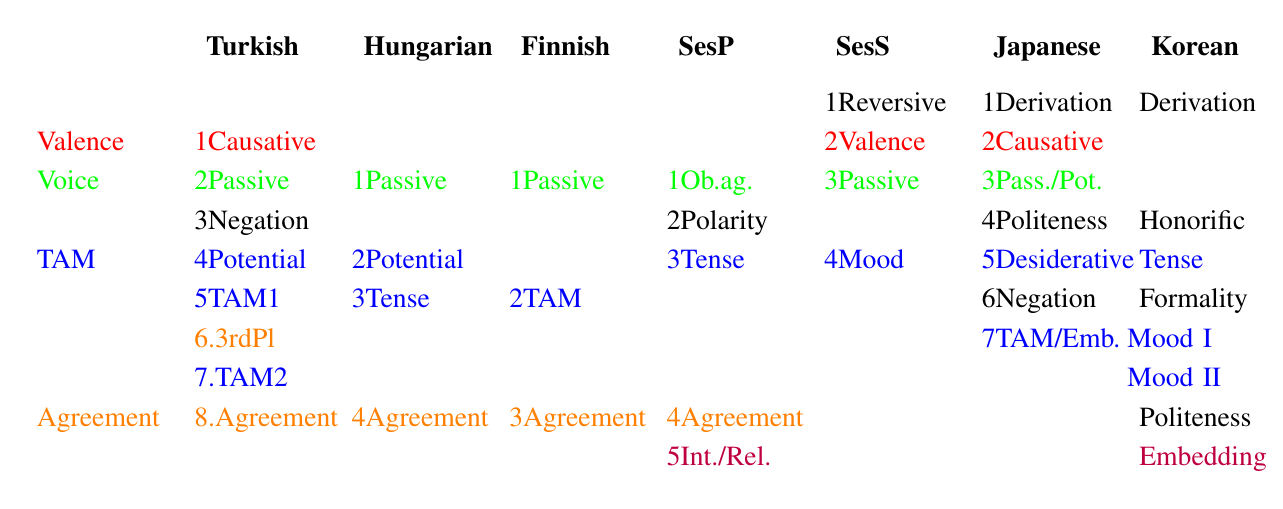
\begin{tikzpicture}[%
% common options for blocks:
block/.style = {draw, fill=blue!30, align=center, anchor=west,
            minimum height=0.65cm, inner sep=0},
% common options for the circles:
ball/.style = {circle, draw, align=center, anchor=north, inner sep=0}]
%\node[rectangle,text width=1.2cm,anchor=base] (A0) at (1,-0.3) {Real};


%\node[rectangle,text width=1.2cm,anchor=base] (A1) at (1,-1.0) {1Derivation};
\node[rectangle,text width=1.2cm,anchor=base, color=red] (A2) at (1,-1.5) {Valence};
\node[rectangle,text width=1.2cm,anchor=base, color=green] (A3) at (1,-2.0) {Voice};
\node[rectangle,text width=1.2cm,anchor=base,color=blue] (A4) at (1,-3) {TAM};
%\node[rectangle,text width=1.2cm,anchor=base,color=blue] (A4) at (1,-3.5) {Tense};
%\node[rectangle,text width=1.2cm,anchor=base,color=blue] (A4) at (1,-4) {Mood};
\node[rectangle,text width=1.2cm,anchor=base,color=orange] (A4) at (1,-5) {Agreement};

% Turkish
\node[rectangle,text width=0.9cm,anchor=base] (B0) at (3,-0.3) {\textbf{Turkish}};
\node[rectangle,text width=1.2cm,anchor=base,color=red] (B1) at (3,-1.5) {1Causative};
\node[rectangle,text width=1.2cm,anchor=base,color=green] (B2) at (3,-2) {2Passive};
\node[rectangle,text width=1.2cm,anchor=base] (B3) at (3,-2.5) {3Negation};
\node[rectangle,text width=1.2cm,anchor=base,color=blue] (B4) at (3,-3) {4Potential};
\node[rectangle,text width=1.2cm,anchor=base,color=blue] (B4) at (3,-3.5) {5TAM1};
\node[rectangle,text width=1.2cm,anchor=base,color=orange] (B4) at (3,-4) {6.3rdPl};
\node[rectangle,text width=1.2cm,anchor=base,color=blue] (B4) at (3,-4.5) {7.TAM2};
\node[rectangle,text width=1.2cm,anchor=base,color=orange] (B4) at (3,-5) {8.Agreement};

% Hungarian
\node[rectangle,text width=0.9cm,anchor=base] (B0) at (5,-0.3) {\textbf{Hungarian}};
\node[rectangle,text width=1.2cm,anchor=base,color=green] (B2) at (5,-2) {1Passive};
\node[rectangle,text width=1.2cm,anchor=base,color=blue] (B4) at (5,-3) {2Potential};
\node[rectangle,text width=1.2cm,anchor=base,color=blue] (B4) at (5,-3.5) {3Tense};
\node[rectangle,text width=1.2cm,anchor=base,color=orange] (B4) at (5,-5) {4Agreement};


% Finnish
\node[rectangle,text width=0.9cm,anchor=base] (B0) at (7,-0.3) {\textbf{Finnish}};
\node[rectangle,text width=1.2cm,anchor=base,color=green] (B2) at (7,-2) {1Passive};
\node[rectangle,text width=1.2cm,anchor=base,color=blue] (B4) at (7,-3.5) {2TAM};
\node[rectangle,text width=1.2cm,anchor=base,color=orange] (B4) at (7,-5) {3Agreement};

% Sesotho Prefixes
\node[rectangle,text width=0.9cm,anchor=base] (B0) at (9,-0.3) {\textbf{SesP}};
\node[rectangle,text width=1.2cm,anchor=base,color=green] (B2) at (9,-2) {1Ob.ag.};
\node[rectangle,text width=1.2cm,anchor=base] (B4) at (9,-2.5) {2Polarity};
\node[rectangle,text width=1.2cm,anchor=base,color=blue] (B4) at (9,-3) {3Tense};
\node[rectangle,text width=1.2cm,anchor=base,color=orange] (B4) at (9,-5) {4Agreement};
\node[rectangle,text width=1.2cm,anchor=base,color=purple] (B4) at (9,-5.5) {5Int./Rel.};

% Sesotho Suffixes
\node[rectangle,text width=0.9cm,anchor=base] (B0) at (11,-0.3) {\textbf{SesS}};
\node[rectangle,text width=1.2cm,anchor=base] (B2) at (11,-1) {1Reversive};
\node[rectangle,text width=1.2cm,anchor=base,color=red] (B2) at (11,-1.5) {2Valence};
\node[rectangle,text width=1.2cm,anchor=base,color=green] (B2) at (11,-2) {3Passive};
\node[rectangle,text width=1.2cm,anchor=base,color=blue] (B4) at (11,-3) {4Mood};



% Japanese
\node[rectangle,text width=0.9cm,anchor=base] (B0) at (13,-0.3) {\textbf{Japanese}};
\node[rectangle,text width=1.2cm,anchor=base] (B2) at (13,-1) {1Derivation};
\node[rectangle,text width=1.2cm,anchor=base,color=red] (B2) at (13,-1.5) {2Causative};
\node[rectangle,text width=1.2cm,anchor=base,color=green] (B2) at (13,-2) {3Pass./Pot.};
\node[rectangle,text width=1.2cm,anchor=base] (B4) at (13,-2.5) {4Politeness};
\node[rectangle,text width=1.2cm,anchor=base,color=blue] (B4) at (13,-3) {5Desiderative};
\node[rectangle,text width=1.2cm,anchor=base] (B4) at (13,-3.5) {6Negation};
\node[rectangle,text width=1.2cm,anchor=base,color=blue] (B4) at (13,-4) {7TAM/Emb.};

% Korean
\node[rectangle,text width=0.9cm,anchor=base] (B0) at (15,-0.3) {\textbf{Korean}};
\node[rectangle,text width=1.2cm,anchor=base] (B2) at (15,-1.0) {Derivation};
\node[rectangle,text width=1.2cm,anchor=base] (B4) at (15,-2.5) {Honorific};
\node[rectangle,text width=1.2cm,anchor=base,color=blue] (B4) at (15,-3) {Tense};
\node[rectangle,text width=1.2cm,anchor=base] (B4) at (15,-3.5) {Formality};
\node[rectangle,text width=1.5cm,anchor=base,color=blue] (B4) at (15,-4.0) {Mood I};
\node[rectangle,text width=1.5cm,anchor=base,color=blue] (B4) at (15,-4.5) {Mood II};
\node[rectangle,text width=1.2cm,anchor=base] (B4) at (15,-5) {Politeness};
\node[rectangle,text width=1.2cm,anchor=base,color=purple] (B4) at (15,-5.5) {Embedding};


%\draw[->] (A1.east) to (B1.west);
%\draw[->] (A2.east) to (B2.west);
%\draw[->] (A3.east) to (B3.west);
%\draw[->] (A4.east) to (B4.west);
\end{tikzpicture}

%    \centering
%\begin{tabular}{l||l|l|l|l|l|l|llll}
%                    & Turkish & Hungarian & Finnish  & Sesotho Pref.     & Ses Suff. & Japanese & Korean\\ \hline\hline
%Derivation          &  &         &          &               & Reversive & suru    & ha,i\\ \hline
%Valence             &  Causative &         &           & Object marker & Valence & Causative\\ \hline
%Voice               & Passive & Passive    & Passive     &               & Passive & Passive\\ \hline
%TAM, Pol.           & Negation  &   Potential  &   Tense/Asp &    Negation &  Politeness &      Potential        & Honorific \\
%                    & Potential & Tense        &    Mood     &     Tense   &    Mood     &   Honorific  &    Tense       \\
%                    &   TAM1    &          &                &         &                  & Tense/Aspect & Formality \\
%                    & lar       &          &           &  & & Negation & Mood I\\
%                    & TAM2         &           &               &          &       &      &  Mood II \\ \hline
%Agreement           & Agreement & Agreement & Agreement & Agreement \\ \hline
%\textit{Other}               & Formality          & Clitic    &              & Int/Rel &      &        & Politeness \\
%                    &           &     &              &  &          &    & Conj \\
%\end{tabular}

\mhahn{TODO make this visually more appealing}

    \caption{Morpheme order across the six languages in our sample, matched with four universal categories (left).}
    \label{tab:table-orders}
\end{figure}


Verbs commonly mark a larger number of inflection categories.
Figure~\ref{tab:table-orders} summarises the affixes in the verbal morphologies of the six morphologically rich languages considered here.
For each language in the sample, we determined a templatic sequence of slots into which morphemes are ordered (see SI Section X for details on how we arrived at these slots).

Verbal affixes are typically grouped into derivational and inflectional affixes.
Derivational affixes derive new verb stems (e.g., 'do' $\rightarrow$ undo), whereas inflectional affixes derive inflected verb forms from verb stems (e.g., `do' $\rightarrow$ `does').
Examples of derivational suffixes are Japanese -su- and Korean -ha-, which derive verbs from non-verbal stems \citep{hasegawa2014japanese, yeon2010korean}.
Another example is the Reversive suffix in Sesotho (corresponding to `un-' in English `do' $\rightarrow$ `undo', \citep{doke1967textbook}).
Derivational affixes generally appear closer to the root than inflectional affixes.

\textit{Valence} affixes (red in Figure~\ref{tab:table-orders}, Example X in Figure~\ref{tab:examples-verbs}) change the number of arguments. A very common type of valence affix is a causative, which adds an argument indicating who causes an event or state to occur \citep{wals-111}.
%In Turkish, -t- marks causatives (\citep{schaaik2020turkish}, Figure~\ref{tab:examples-verbs}).
\textit{Voice} (green in Figure~\ref{tab:table-orders}) describes the distinction between active and passive (CITE). An example is the Japanese passive suffix -\textit{(r)are}- (Figure~\ref{tab:examples-verbs}).
\textit{Tense-Aspect-Mood (TAM)} (blue in Figure~\ref{tab:table-orders}) comprises three types of categories.
\textit{Aspect} describes how an event unfolds over time \citep{comrie1976aspect,dahl1985tense,binnick1991time}.
An example of aspect marking is the English progressive \textit{to be} ...-\textit{ing}, which indicates that an action is currently ongoing (CITE).
\textit{Tense} describes where an event is located in time (e.g. past or future, CITE).
Aspect and tense categories are often fused in morphology \citep{binnick2012the}, and this also applies to the languages in our sample.
Examples of tense and aspect marking are shown in Figure~\ref{tab:examples-verbs}.
\textit{Mood} describes a relation between an event and the speaker, including an assessment of the event's reality \cite{palmer1986mood,portner2018mood}.
In analytical languages such as English, mood distinctions are often indicated using verbs such as \textit{might} or adverbs such as \textit{possibly}.
A common mood category is the Potential mood, which indicates possibility (Turkish, Hungarian).
Figure~\ref{tab:examples-verbs} shows how it is marked morphologically with -het- in Hungarian \citep{rounds2001hungarian}.
In many languages, mood marking is at least partically fused with tense and aspect; for instance, the Japanese suffix -\textit{yoo} can mark future tense and the hortative mood (`let's ...', \citep{hasegawa2014japanese}).
Tense, aspect, mood are often together referred to as TAM (Tense-Aspect-Mood, \citep{bybee1994the, wals-69}).
Some languages have a single affix slot that accommodates a fused morpheme indicating TAM.
For instance, Finnish marks both tense (present and past) and mood (indicative, conditional, and potential) categories with a single morpheme in the slot labeled TAM.
Other languages have multiple slots, for instance, Turkish has (TODO explain TAM1, TAM2).
\textit{Subject agreement} (orange in Figure~\ref{tab:table-orders}) mark categories of the subject, most often its person and number, sometimes also other categories such as its gender.
An example is English third-person -s.
% re agreement for references: http://epubs.surrey.ac.uk/1063/1/fulltext.pdf
In our sample, Turkish, Hungarian, Finnish, and Sesotho have a subject agreement slot (Figure~\ref{tab:table-orders}); Turkish also has a special slot occupied only by the third-person plural marker \textit{-lar-} (indicated as 3rdPl in ~\ref{tab:table-orders}).

The ordering of morphemes encoding these categories shows universal tendencies \citep{bybee-morphology-1985}, which we summarize as follows:


\begin{adjustwidth}{6em}{6em}
\textsc{Verb Affix Ordering} \citep{bybee-morphology-1985}:
Verb affixes are ordered as follows, outward from the verb stem:

\begin{tabular}{llllllllllllllllllllllllll}
verb stem & valence & voice & TAM & subject agreement
\end{tabular}
\end{adjustwidth}

%Based on data from several dozens of languages, \citep{bybee-morphology-1985} proposes the following ordering of these common verb affixes:
%\begin{quote}
%\begin{tabular}{llllllllllllllllllllllllll}
%verb stem & valence & voice & aspect & tense& mood & subject agreement
%\end{tabular}
%\end{quote}

Figure~\ref{tab:table-orders} shows that the languages in our sample largely support this universal, with the exception of the order of the special third-plural suffix slot in Turkish, which intervenes between two TAM slots.
\citet{bybee-morphology-1985} also provides evidence for ordering preferences within aspect, tense, and mood; however, we do not distinguish between them as these are frequently fused in languages.


While these are particularly common types of affixes, there are further types, some of which occur in the six languages of our sample.
While agreement is most commonly established with the subject, \textit{agreement with the object} is found in Sesotho \citep{doke1967textbook} (in person and noun class) and in Hungarian \citep{rounds2001hungarian} (in definiteness); it is fused with subject agreement in the latter case.
\textit{Polarity} refers to the opposition between affirmative (e.g. `she arrived') and negative  (e.g., `she did not arrive') statements \citep{wals-112}.
\textit{Evidentiality} indicates on what evidence a speaker bases an assertion \citep{aikhenvald2003evidentiality}.
\textit{Formality}, \text{honorifics}, and \text{politeness} are categories that index social relations between the speaker, the addressee, and the topic of the conversation (CITE).
In our sample, these are prominent in Korean and Japanese.
The Japanese politeness marker -masu- and the Korean formality (-p) and politeness (-yo) suffixes index the social relation between the speaker and the addressee \citep{hasegawa2014japanese, yeon2010korean}; the Korean honorific suffix -si- indexes the social relation between the speaker and the topic of the conversation \citep{yeon2010korean}.

Furthermore, verb forms can have affixes indicating the syntactic position of the verb within a sentence, in particular, affixes marking infinitives or other nonfinite forms.
We use the term \textit{Embedding} (TODO) for this type of morpheme.


%We focus on inflection, except in those cases where derivational affixes are clearly marked in available data.
%Inflectional suffixes are generally outside of derivational affixes

% somewhere explain the choice of languages
% - rich agglutinative.
% - must have data with suitable morphological analysis.
% - Among the languages, Hungarian and Finnish are genetically related (X millenia). There is also some evidence for genetic relations beyond these (Japanese, Korean, Turkish), but such relations would have to be quite ancient (x millenia).
% The morphemes found in these languages as considered here are generally not cognate.





\section{Methods}

\subsection{Data} % TODO: Becky
% why agglutinative?


We obtained data from four morphologically rich languages.
We focused on languages in which verbs and nouns often have more than two morphemes per words, as that allows us to test predictions about the relative ordering of different morphemes.
Furthermore, we focused on languages in which the morphemes within a word have clearly delimited boundaries, providing unambiguous information about the ordering of morphemes.
Languages with these properties are referred to as agglutinative.
Mutual information depends on the frequencies at which different morphological forms are used. We thus selected agglutinative languages for which large-scale text corpora with morphological annotation was available.
The language sample includes Universal Dependencies (UD) corpora for Korean \citep{chun2018building}, Turkish \citep{turkish-imst}, Hungarian \citep{hungarian-szeged}, and Finnish \citep{UDFinnish-TDT}.
In addition, we also reanalyze the data from \citet{Hahn2020modeling}, covering UD data for Japanese \citep{asahara2018universal} and the Child Language Data Exchange System (CHILDES) Sesotho corpus \citep{demuth1992acquisition} in a way consistent with our analysis of the other four languages.


\mhahn{TODO corpus sizes.}


For nouns, we focused on Turkish, Hungarian, and Finnish, as nouns in these languages often have more than one affix.
We used all six languages for verbs.

For each language, we selected nouns and verbs based on the part-of-speech annotation in each corpus.
We then identified which morphemes each extracted word was composed of, on the basis of the annotation provided in the corpora (see SI Appendix, Section X for details).



\subsection{Setup}
For estimating memory-surprisal tradeoffs, we modeled words as strings of morphemes, following \citet{Hahn2020modeling}.
For instance, we represent \textit{juttu-i-hi-si} `into your stories' (Figure REF) as juttu-\textsc{Plural}-\textsc{Illative}-\textsc{2sgPoss}.
(See SI Appendix Section X for experiments taking morphophonological interactions between morphemes into account.)

For each language, we parameterize possible morpheme orderings through the $N!$ possible orderings of the $N$ slots.
Applying any such ordering to the forms extracted from the corpus results in a set of counterfactual forms with some associated memory-surprisal tradeoff curve; in particular, applying the real orderings (Figure REF) results in the actual morpheme sequences as found in the corpus.
Following \citet{Hahn2020modeling}, we quantify the efficiency of a tradeoff curve using its Area under the Curve (AUC). Lower values of AUC indicate a steeper decay of mutual information, and thus a more efficient tradeoff.

We compare the real orderings (\textit{real}) to three different kinds of alternative orderings: randomized morpheme orderings (\textit{random}), the reversed real orderings (\textit{reverse}), and morpheme orderings that are optimized to minimize AUC under the tradeoff curve (\textit{optimized}). 

We estimated memory-surprisal tradeoffs and computationally optimized orderings for the AUC under the tradeoff curve using the method of \citet{Hahn2020modeling}.



%\subsection{Nouns}
%\mhahn{Here is an idea for how we might structure this section: We can describe the systems in the individual languages in prose and in broad strokes here, highlighting what's common and what's different across languages. For the nouns, it's interesting to point out that the relative position of Case and Possessor differs between Finnish and the rest, whereas the position of Number is stable. For the verbs, the discussion could refer to Table~\ref{tab:table-orders}. I've collapsed all the Tense/Aspect/Modality/Negation morphemes into one big category ``TAM, Polarity'' since aligning the morphemes in each language with those individual categories seems very hard, and in any case there are differences between the languages. Talking about this in broad strokes, again highlighting parallels and differences, should be the right level of detail here. You can draw on Table S1 and Tables S5, S12, S13 in the appendix for my revised verb morpheme segmentation in Korean, Turkish, and Hungarian. We can then leave precise and detailed discussion of each of the languages, including detailed references to the literature for these individual languages, to the appendix. The \texttt{enumerate} blocks could go into the appendix, with some description of what each morpheme does and references to reference grammars (I can do this).}
%We're interested in investigating languages where nouns are inflected with multiple suffixes, because that allows us to more extensively measure the relationship between mutual information and mutual information. As such, we only investigated our hypothesis on Turkish, Hungarian, and Finnish nouns. All of these languages inflect nouns for number, possessor person, possessor number, and case, in that order. Finnish is the exception, where we include derivation (verbs that are nominalized, for example), and where the possessor person and number appears after the case suffix in the natural ordering. 
%In contrast, the number suffix, which is generally only marked for the plural, has a stable position close to the root in all three languages. Number has high mutual information with the noun root, because certain nouns have a tendency to appear only in the plural or only in the singular. As such, number must come close to the root.
%\subsection{Verbs}
%For verbs, we investigated Finnish, Hungarian, Japanese, Korean, Sesotho, and Turkish inflectional suffixes. Broadly speaking, all of the languages have a real ordering of valence, voice, negation, tense/aspect/mood (TAM), person and number, and formality, where applicable. \becky{TODO: Check that this is correct and discuss some specifics.} 
%\becky{Which language provides data for which kind of suffix?}
%Following \citet{Hahn2020modeling}, we compare the efficiency each natural language's morpheme orderings (\textit{real}) to three different kinds of baselines: randomized morpheme orderings (\textit{random}), the reversed natural orderings (\textit{reverse}), and morpheme orderings that are optimized to maximize MI (\textit{optimized}). 


%https://en.wiktionary.org/wiki/%EB%B0%94%EB%9D%BC%EB%8B%A4

\section{Results}
Figures \ref{fig:auc_verbs} and \ref{fig:auc_nouns} show area under the curve (AUC) plots for random orders as compared to the real, natural order of morphemes for verbs and nouns, respectively.
%Here, AUC refers to the area under the curve for the memory-surprisal tradeoff for each order, where the lower the AUC is, the more efficient that memory-surprisal tradeoff is.
Across languages, and for both nouns and verbs, real orderings (TODO color) have lower AUC than most random baseline orderings (TODO stats), close to the computationally optimized orderings (TODO color) meaning that they enable more efficient memory-surprisal tradeoffs than most of the $N!$ possible orderings. 

Second, we evaluated to what extent real and optimized orderings agree in the orderings that they define, compared to the agreement between real and random orderings.
Table \ref{tab:optimized_acc} shows the agreement of optimized and random baseline orderings with real orderings.
We defined three measures of agreement:
\textit{Pairs} counts what fraction of all pairs of affixes within a single word from the corpus are ordered in the same relative order under both orderings.
\textit{Full} counts what fraction of words from the corpus is ordered entirely identically under both orderings.
Finally, \textit{Full (Types)} is analogous to \textit{Full} but only counts words that appear multiple times only once, in order to control for the possible effect of individual highly frequent forms.


For nouns, the agreement between real and optimized orderings is perfect, far above the agreement with baseline grammars (TODO stats. how many baseline grammars are outperformed by optimized?).
For verbs, agreement between real and optimized orderings is above 90\% for Hungarian, Turkish, Korean, Japanese, and Sesotho prefixes (TODO stats).
For Sesotho suffixes, agreement is lower, though still better than X\% of baselines.
In Finnish, agreement between real and optimzed orderings is similar to agreement between real and baseline orderings (see below for discussion).

Figures \ref{fig:real_and_optimized_nouns} and \ref{fig:real_and_optimized_verbs} directly compare real and optimized orderings for nouns and verbs respectively.
The real and optimized noun orders show a perfect match.
In particular, Greenberg's Universal (TODO) is recovered by all optimized orderings.
The real and verb optimized orders show some disagreement in each language.
%Divergences in the real and optimized verbal morpheme orders will be analyzed more in the Discussion section. 

%\becky{Refer to S3 to introduce this paragraph}
Figure \ref{fig:optimized_and_universal_orders} compares the universal verb morpheme ordering to the optimized ordering for each language.
Hungarian, Japanese, Korean, and Sesotho (suffixes and prefixes) match the universal ordering perfectly for the morphemes occurring in each of these languages. 
Turkish matches the universal order except for the 3rd person plural agreement marker ``-lar-'', which is separated from the other agreement morphemes in both real and optimized orderings.
For Finnish, the optimized order is the same as the universal order except for the fact that the agreement marker comes closest to the root instead of furthest, which accounts for the low quantitative agreement observed in Table~\ref{tab:optimized_acc}.
This can be traced to a peculiarity of the Finnish passive, which uses a single agreement marker that is only used for passives, and which does not distinguish between person and number categories (referred to as impersonal by \citep[Section 69]{karlsson1999finnish}).
This means that the agreement marker has substantial mutual information with the voice morpheme, so that optimized orderings prefer agreement and voice morphemes to be adjacent.
On active forms -- which, unlike the passive, are fully inflected for person and number -- optimized orderings place the agreement slot after the TAM slot, in agreement with the real ordering.

%Taking a step back and looking at all of these languages at a whole, we see that the languages' optimized orders tend to closely mirror Bybee's universal ordering, which also means that these languages also have a high level of agreement between them on the relative ordering of verbal morphemes. As such, it's possible to predict Bybee's universal ordering from looking at commonalities between optimized orders of natural languages. 


%\becky{conclude}

\begin{figure}
    \centering
    \begin{tabular}{cccccc}
    \textsc{Finnish} & \textsc{Turkish} & \textsc{Hungarian} \\
        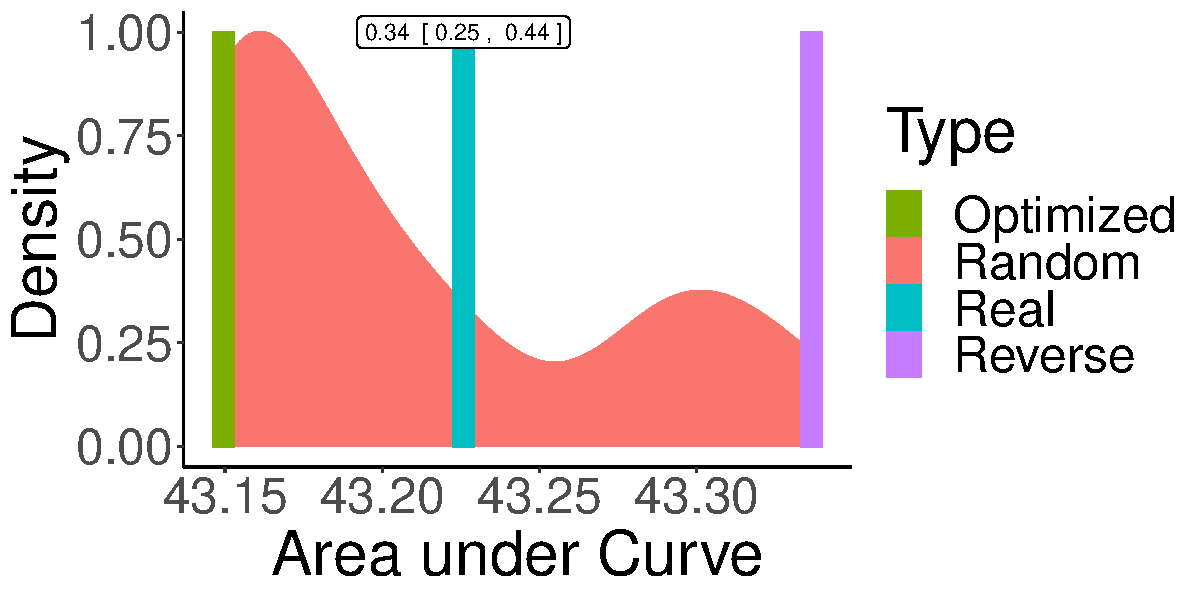
\includegraphics[width=0.3\textwidth]{figures/finnish_verbs/suffixes-byMorphemes-auc-hist-heldout-Coarse-FineSurprisal-optimized.pdf}
        &
    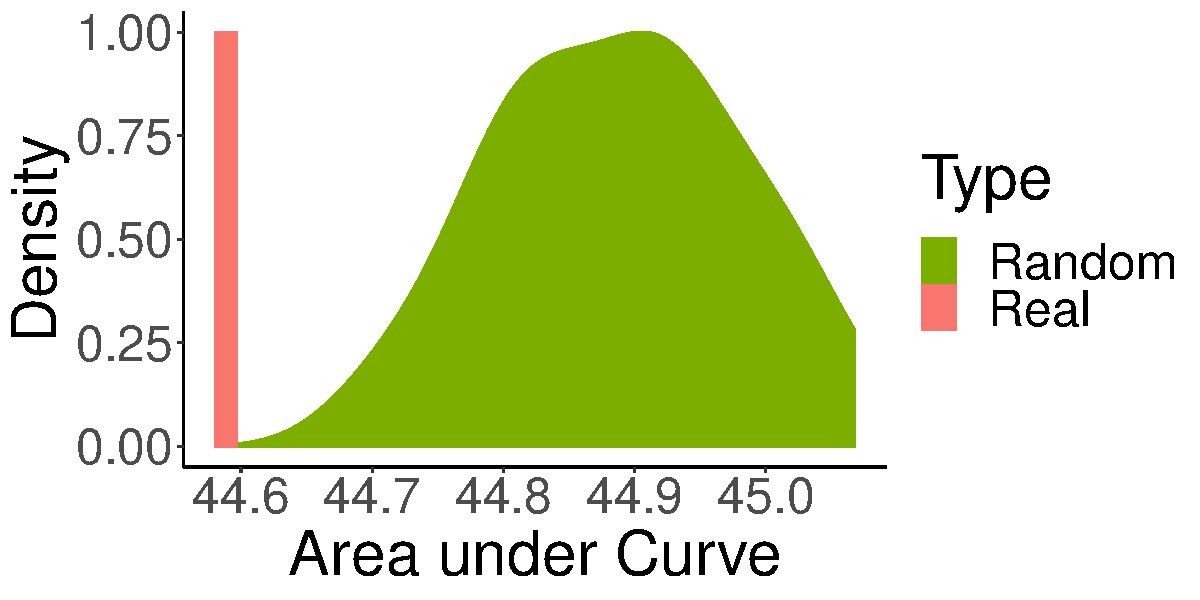
\includegraphics[width=0.3\textwidth]{figures/turkish_verbs/suffixes-byMorphemes-auc-hist-heldout-Coarse-FineSurprisal-optimized.pdf}
    &
    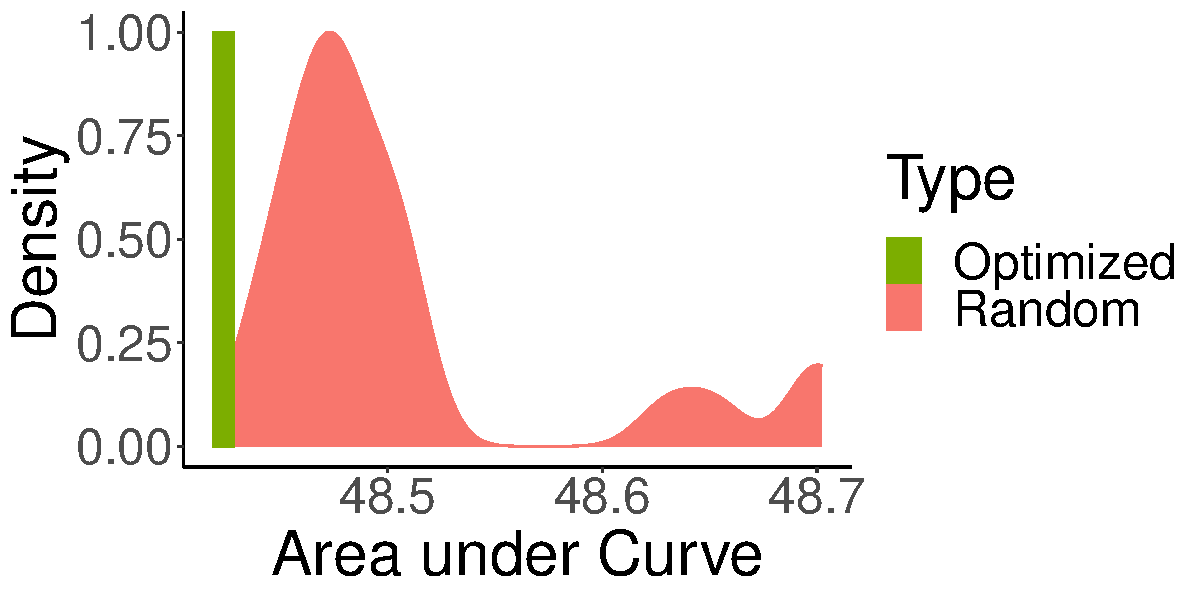
\includegraphics[width=0.3\textwidth]{figures/hungarian_verbs/suffixes-byMorphemes-auc-hist-heldout-Coarse-FineSurprisal-optimized.pdf}
    \\
    \textsc{Korean} & \textsc{Japanese} & \textsc{Sesotho Prefixes} \\
    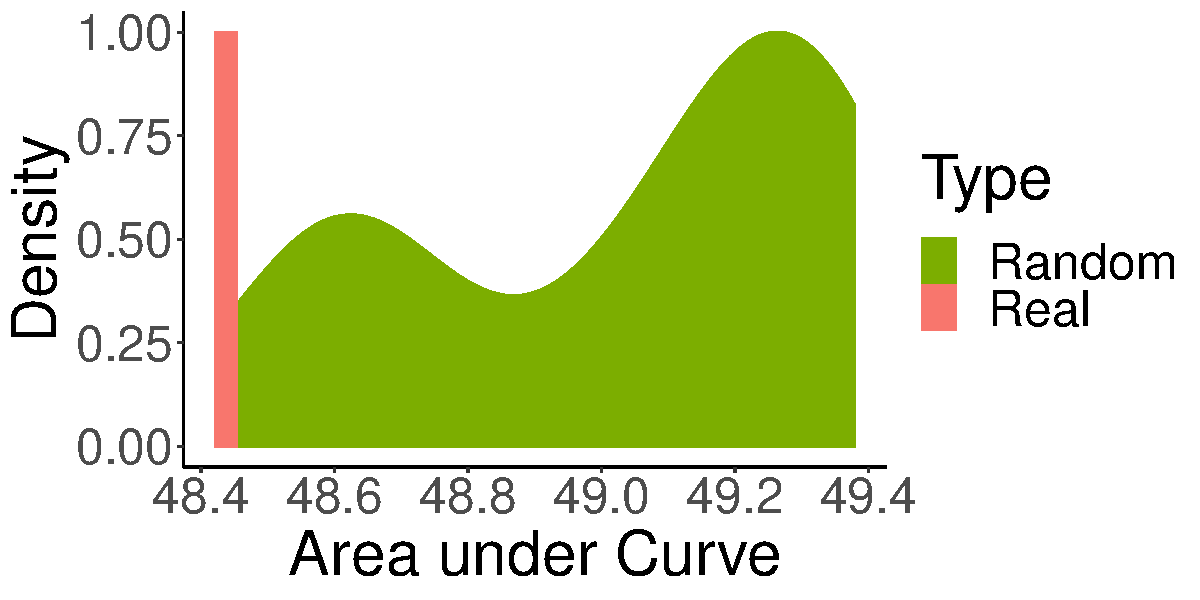
\includegraphics[width=0.3\textwidth]{figures/korean/suffixes-byMorphemes-auc-hist-heldout-Coarse-FineSurprisal-optimized.pdf}
    &
        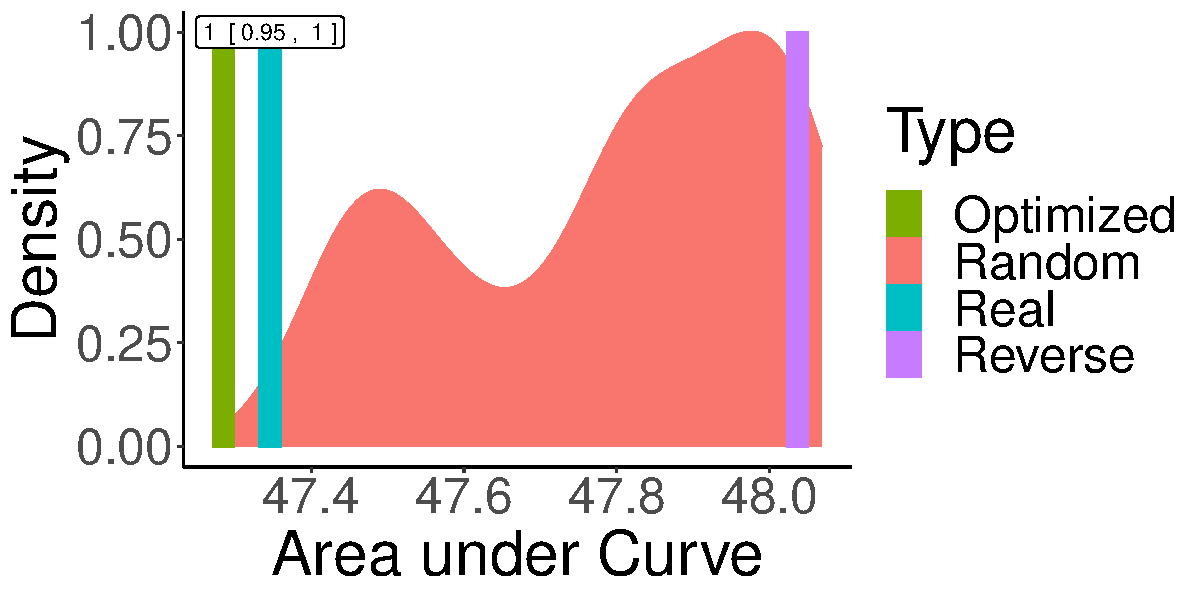
\includegraphics[width=0.3\textwidth]{figures/japanese/suffixes-byMorphemes-auc-hist-heldout-Coarse-FineSurprisal-optimized.pdf}
        &
            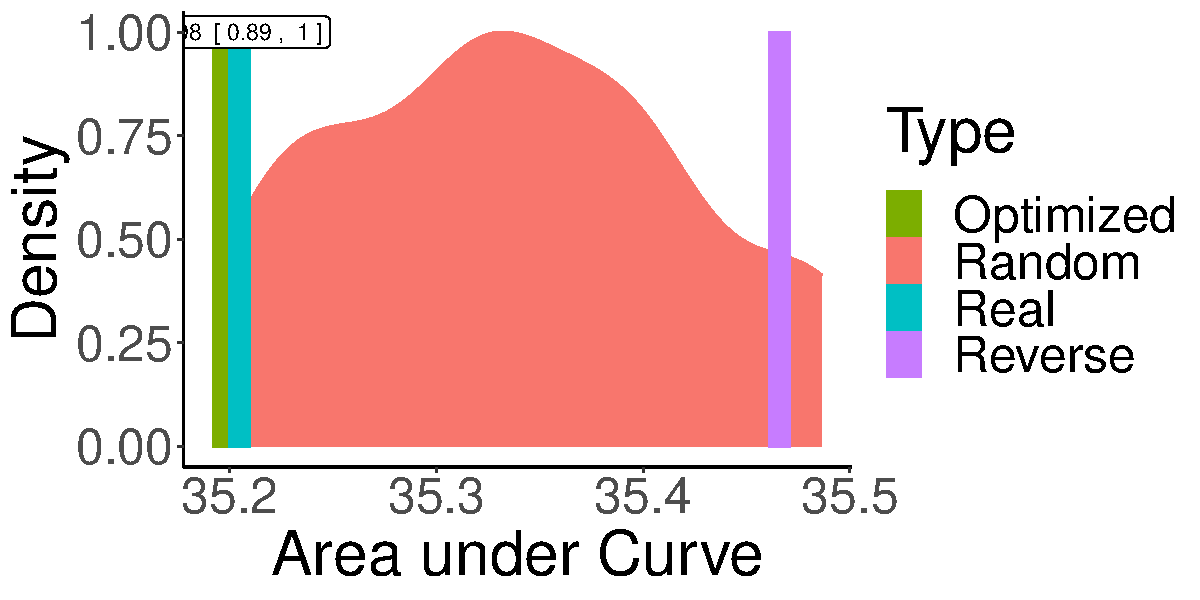
\includegraphics[width=0.3\textwidth]{figures/sesotho_prefixes/suffixes-byMorphemes-auc-hist-heldout-Coarse-FineSurprisal-optimized.pdf}
            \\
            \textsc{Sesotho Suffixes} \\
            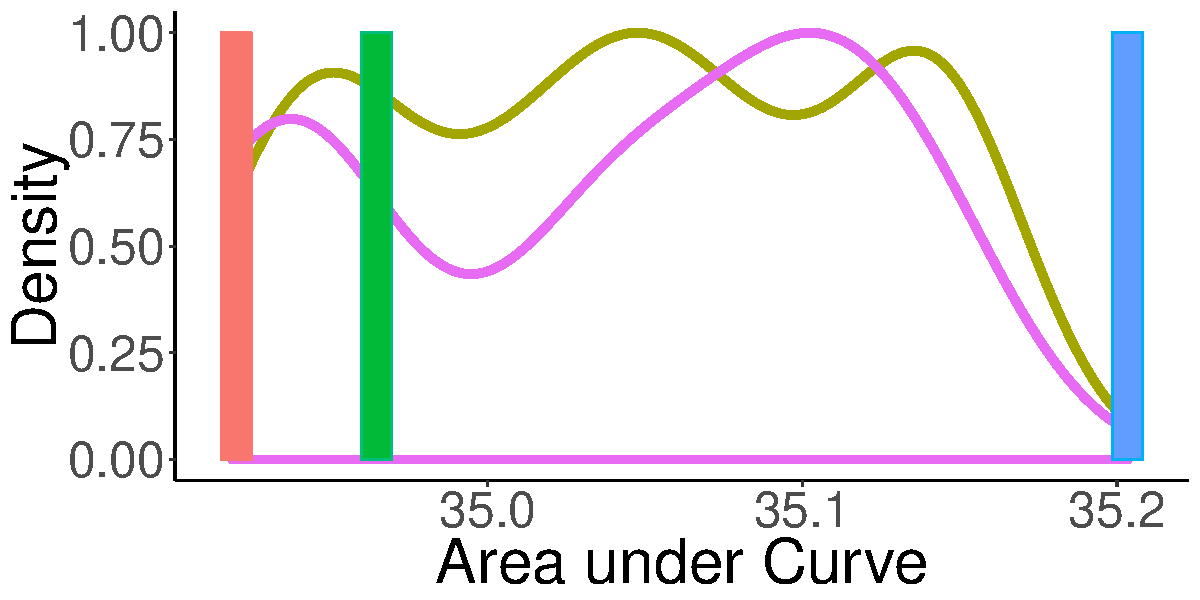
\includegraphics[width=0.3\textwidth]{figures/sesotho_suffixes/suffixes-byMorphemes-auc-hist-heldout-Coarse-FineSurprisal-optimized.pdf}
    \end{tabular}

    
    \caption{AUC Histograms for Verb Affixes.}
    \label{fig:auc_verbs}
\end{figure}


\begin{figure}
\begin{tabular}{ccc}
\textsc{Finnish} & \textsc{Turkish} & \textsc{Hungarian} \\
    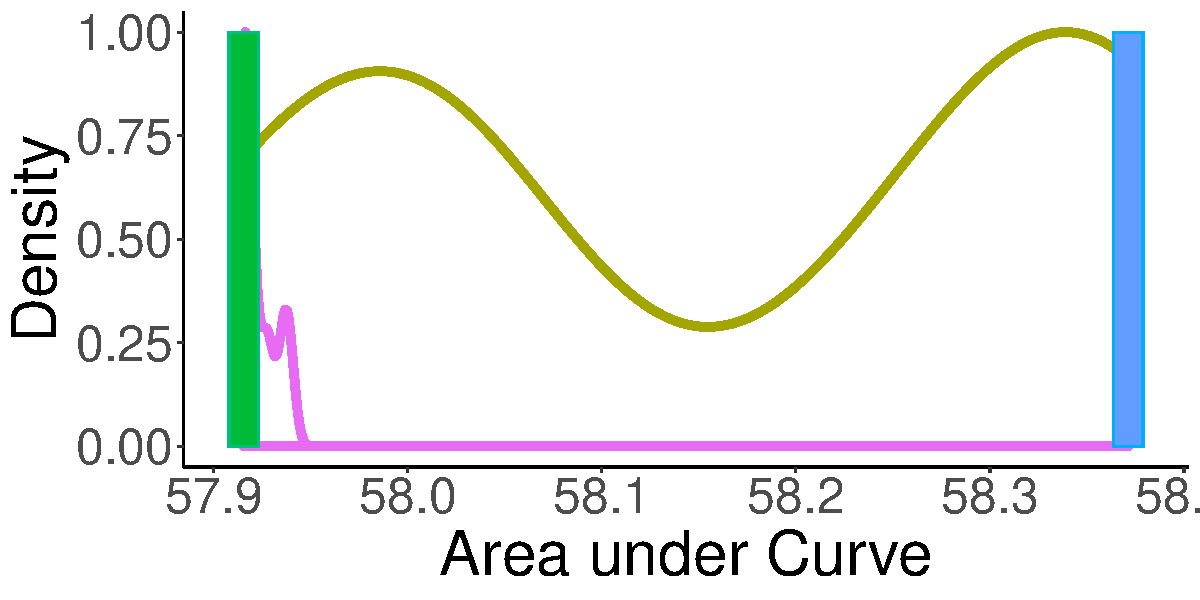
\includegraphics[width=0.3\textwidth]{figures/finnish_nouns/suffixes-byMorphemes-auc-hist-heldout-Coarse-FineSurprisal-optimized.pdf}
    &
    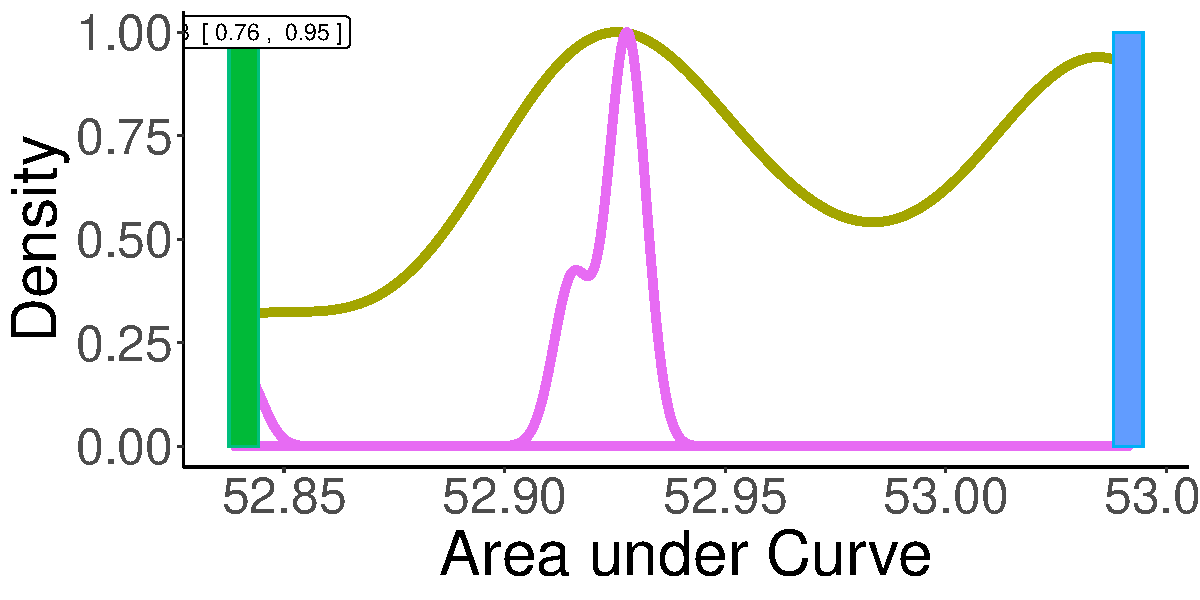
\includegraphics[width=0.3\textwidth]{figures/turkish_nouns/suffixes-byMorphemes-auc-hist-heldout-Coarse-FineSurprisal-optimized.pdf}
    &
    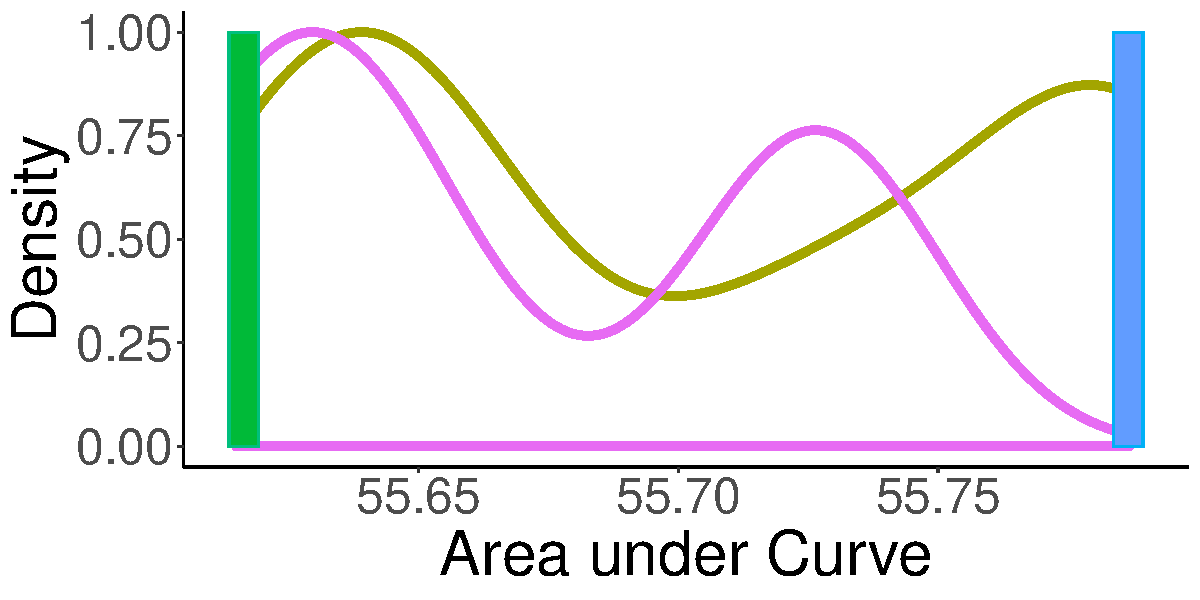
\includegraphics[width=0.3\textwidth]{figures/hungarian_nouns/suffixes-byMorphemes-auc-hist-heldout-Coarse-FineSurprisal-optimized.pdf}
    \end{tabular}
    \caption{Noun Suffixes}
    \label{fig:auc_nouns}
\end{figure}

\begin{table}[]
    \centering
    \begin{tabular}{l|l|ll|lllllllll}
    &     &    \multicolumn{2}{c|}{Pairs} & \multicolumn{2}{c|}{Full} & \multicolumn{2}{c}{Full (Types)} \\
     &   &     Optim. & Baseline & Optim. & Baseline & Optim. & Baseline \\ \hline
 & finnish nouns & 1.0 (0.0) & 0.42 (0.31) & 1.0 (0.0) & 0.37 (0.32) & 1.0 (0.0) & 0.38 (0.29) \\
 & turkish nouns & 1.0 (0.0) & 0.56 (0.36) & 1.0 (0.0) & 0.5 (0.37) & 1.0 (0.0) & 0.5 (0.36) \\
 & hungarian nouns & 1.0 (0.0) & 0.48 (0.22) & 1.0 (0.0) & 0.33 (0.27) & 1.0 (0.0) & 0.33 (0.27) \\
 \hline
 & finnish verbs & 0.4 (0.3) & 0.4 (0.37) & 0.38 (0.31) & 0.39 (0.38) & 0.36 (0.32) & 0.38 (0.37) \\
 & hungarian verbs & 0.95 (0.09) & 0.52 (0.37) & 0.95 (0.0) & 0.5 (0.4) & 0.94 (0.0) & 0.5 (0.39) \\
 & turkish verbs & 0.96 (0.09) & 0.46 (0.14) & 0.95 (0.0) & 0.37 (0.15) & 0.93 (0.07) & 0.36 (0.14) \\
 & korean & 0.97 (0.1) & 0.56 (0.33) & 0.97 (0.0) & 0.53 (0.33) & 0.95 (0.0) & 0.53 (0.36) \\
 & japanese & 0.94 (0.08) & 0.48 (0.24) & 0.93 (0.0) & 0.39 (0.24) & 0.9 (0.1) & 0.39 (0.24) \\
 & sesotho prefixes & 0.99 (0.0) & 0.5 (0.48) & 0.99 (0.0) & 0.5 (0.48) & 0.98 (0.0) & 0.51 (0.46) \\
 & sesotho suffixes & 0.62 (0.0) & 0.48 (0.2) & 0.54 (0.0) & 0.45 (0.19) & 0.52 (0.0) & 0.44 (0.19) \\
    \end{tabular}
    \caption{Accuracies in predicting morpheme ordering. `Optim.' indicates grammars optimized for AUC, `'Baseline' indicates randomly constructed weights.
    In each cell, we provide the mean and the stgandard deviation over orderings. `Pairs' indicates the fraction of pairs of morphemes occurring together in the same word that are ordered correctly. `Full' indicates the fraction of verb forms in the corpus that are ordered fully correctly. `Full (Types)' counts forms that occur multiple times only once, it thus down-weights the role of frequent forms.}
    \label{tab:optimized_acc}
\end{table}



\begin{figure}[]
\begin{tabular}{cccccccc}
\textsc{Turkish} & \textsc{Hungarian} & \textsc{Finnish} \\
\begin{minipage}{.3\textwidth}
    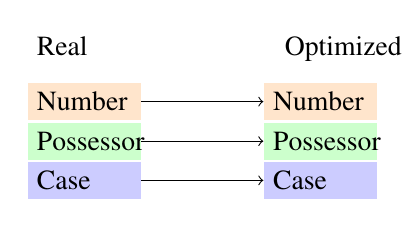
\begin{tikzpicture}[%
% common options for blocks:
block/.style = {draw, fill=blue!30, align=center, anchor=west,
            minimum height=0.65cm, inner sep=0},
% common options for the circles:
ball/.style = {circle, draw, align=center, anchor=north, inner sep=0}]
\node[rectangle,text width=1.2cm,anchor=base] (A0) at (1,-0.3) {Real};
\node[rectangle,text width=0.9cm,anchor=base] (B0) at (4,-0.3) {Optimized};
\node[rectangle,text width=1.2cm,anchor=base, fill=orange!20] (A1) at (1,-1.0) {Number};
\node[rectangle,text width=1.2cm,anchor=base, fill=green!20] (A2) at (1,-1.5) {Possessor};
\node[rectangle,text width=1.2cm,anchor=base, fill=blue!20] (A3) at (1,-2.0) {Case};
\node[rectangle,text width=1.2cm,anchor=base, fill=orange!20] (B1) at (4,-1.0) {Number};
\node[rectangle,text width=1.2cm,anchor=base, fill=green!20] (B2) at (4,-1.5) {Possessor};
\node[rectangle,text width=1.2cm,anchor=base, fill=blue!20] (B3) at (4,-2.0) {Case};
\draw[->] (A1.east) to (B1.west);
\draw[->] (A2.east) to (B2.west);
\draw[->] (A3.east) to (B3.west);
\end{tikzpicture}

    \end{minipage}
  &
  \begin{minipage}{.3\textwidth}
    \begin{tikzpicture}[%
% common options for blocks:
block/.style = {draw, fill=blue!30, align=center, anchor=west,
            minimum height=0.65cm, inner sep=0},
% common options for the circles:
ball/.style = {circle, draw, align=center, anchor=north, inner sep=0}]
\node[rectangle,text width=1.2cm,anchor=base] (A0) at (1,-0.3) {Real};
\node[rectangle,text width=0.9cm,anchor=base] (B0) at (4,-0.3) {Optimized};
\node[rectangle,text width=1.2cm,anchor=base] (A1) at (1,-1.0) {Number};
\node[rectangle,text width=1.2cm,anchor=base] (A2) at (1,-1.5) {Psor_person};
\node[rectangle,text width=1.2cm,anchor=base] (A3) at (1,-2.0) {Psor_number};
\node[rectangle,text width=1.2cm,anchor=base] (A4) at (1,-2.5) {Case};
\node[rectangle,text width=1.2cm,anchor=base] (B1) at (4,-1.0) {Number};
\node[rectangle,text width=1.2cm,anchor=base] (B2) at (4,-1.5) {Psor_person};
\node[rectangle,text width=1.2cm,anchor=base] (B3) at (4,-2.0) {Psor_number};
\node[rectangle,text width=1.2cm,anchor=base] (B4) at (4,-2.5) {Case};
\draw[->] (A1.east) to (B1.west);
\draw[->] (A2.east) to (B2.west);
\draw[->] (A3.east) to (B3.west);
\draw[->] (A4.east) to (B4.west);
\end{tikzpicture}

    \end{minipage}
  &
  \begin{minipage}{.3\textwidth}
    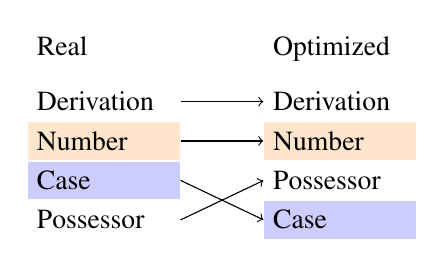
\begin{tikzpicture}[%
% common options for blocks:
block/.style = {draw, fill=blue!30, align=center, anchor=west,
            minimum height=0.65cm, inner sep=0},
% common options for the circles:
ball/.style = {circle, draw, align=center, anchor=north, inner sep=0}]
\node[rectangle,text width=1.7cm,anchor=base] (A0) at (1,-0.3) {Real};
\node[rectangle,text width=1.7cm,anchor=base] (B0) at (4,-0.3) {Optimized};
\node[rectangle,text width=1.7cm,anchor=base] (A1) at (1,-1.0) {Derivation};
\node[rectangle,text width=1.7cm,anchor=base, fill=orange!20] (A2) at (1,-1.5) {Number};
\node[rectangle,text width=1.7cm,anchor=base, fill=blue!20] (A3) at (1,-2.0) {Case};
\node[rectangle,text width=1.7cm,anchor=base] (A4) at (1,-2.5) {Possessor};
\node[rectangle,text width=1.7cm,anchor=base] (B1) at (4,-1.0) {Derivation};
\node[rectangle,text width=1.7cm,anchor=base, fill=orange!20] (B2) at (4,-1.5) {Number};
\node[rectangle,text width=1.7cm,anchor=base] (B3) at (4,-2.0) {Possessor};
\node[rectangle,text width=1.7cm,anchor=base, fill=blue!20] (B4) at (4,-2.5) {Case};
\draw[->] (A1.east) to (B1.west);
\draw[->] (A2.east) to (B2.west);
\draw[->] (A3.east) to (B4.west);
\draw[->] (A4.east) to (B3.west);
\end{tikzpicture}

  \end{minipage}
  \end{tabular}
  
    \caption{Real and optimized ordering (nouns)}
    \label{fig:real_and_optimized_nouns}
\end{figure}


\begin{figure}[]

\begin{tabular}{cccccccc}
\textsc{Turkish} & \textsc{Hungarian} & \textsc{Finnish} \\
\begin{minipage}{.3\textwidth}
    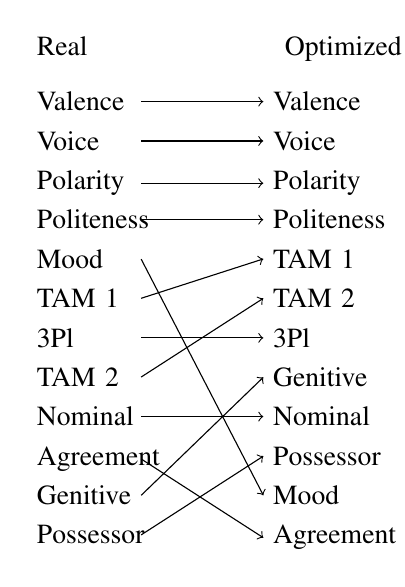
\begin{tikzpicture}[%
% common options for blocks:
block/.style = {draw, fill=blue!30, align=center, anchor=west,
            minimum height=0.65cm, inner sep=0},
% common options for the circles:
ball/.style = {circle, draw, align=center, anchor=north, inner sep=0}]
\node[rectangle,text width=1.2cm,anchor=base] (A0) at (1,-0.3) {Real};
\node[rectangle,text width=0.9cm,anchor=base] (B0) at (4,-0.3) {Optimized};
\node[rectangle,text width=1.2cm,anchor=base] (A1) at (1,-1.0) {Valence};
\node[rectangle,text width=1.2cm,anchor=base] (A2) at (1,-1.5) {Voice};
\node[rectangle,text width=1.2cm,anchor=base] (A3) at (1,-2.0) {Polarity};
\node[rectangle,text width=1.2cm,anchor=base] (A4) at (1,-2.5) {Politeness};
\node[rectangle,text width=1.2cm,anchor=base] (A5) at (1,-3.0) {Mood};
\node[rectangle,text width=1.2cm,anchor=base] (A6) at (1,-3.5) {TAM 1};
\node[rectangle,text width=1.2cm,anchor=base] (A7) at (1,-4.0) {3Pl};
\node[rectangle,text width=1.2cm,anchor=base] (A8) at (1,-4.5) {TAM 2};
\node[rectangle,text width=1.2cm,anchor=base] (A9) at (1,-5.0) {Nominal};
\node[rectangle,text width=1.2cm,anchor=base] (A10) at (1,-5.5) {Agreement};
\node[rectangle,text width=1.2cm,anchor=base] (A11) at (1,-6.0) {Genitive};
\node[rectangle,text width=1.2cm,anchor=base] (A12) at (1,-6.5) {Possessor};
\node[rectangle,text width=1.2cm,anchor=base] (B1) at (4,-1.0) {Valence};
\node[rectangle,text width=1.2cm,anchor=base] (B2) at (4,-1.5) {Voice};
\node[rectangle,text width=1.2cm,anchor=base] (B3) at (4,-2.0) {Polarity};
\node[rectangle,text width=1.2cm,anchor=base] (B4) at (4,-2.5) {Politeness};
\node[rectangle,text width=1.2cm,anchor=base] (B5) at (4,-3.0) {TAM 1};
\node[rectangle,text width=1.2cm,anchor=base] (B6) at (4,-3.5) {TAM 2};
\node[rectangle,text width=1.2cm,anchor=base] (B7) at (4,-4.0) {3Pl};
\node[rectangle,text width=1.2cm,anchor=base] (B8) at (4,-4.5) {Genitive};
\node[rectangle,text width=1.2cm,anchor=base] (B9) at (4,-5.0) {Nominal};
\node[rectangle,text width=1.2cm,anchor=base] (B10) at (4,-5.5) {Possessor};
\node[rectangle,text width=1.2cm,anchor=base] (B11) at (4,-6.0) {Mood};
\node[rectangle,text width=1.2cm,anchor=base] (B12) at (4,-6.5) {Agreement};
\draw[->] (A1.east) to (B1.west);
\draw[->] (A2.east) to (B2.west);
\draw[->] (A3.east) to (B3.west);
\draw[->] (A4.east) to (B4.west);
\draw[->] (A5.east) to (B11.west);
\draw[->] (A6.east) to (B5.west);
\draw[->] (A7.east) to (B7.west);
\draw[->] (A8.east) to (B6.west);
\draw[->] (A9.east) to (B9.west);
\draw[->] (A10.east) to (B12.west);
\draw[->] (A11.east) to (B8.west);
\draw[->] (A12.east) to (B10.west);
\end{tikzpicture}

  \end{minipage}
  &
  \begin{minipage}{.3\textwidth}
    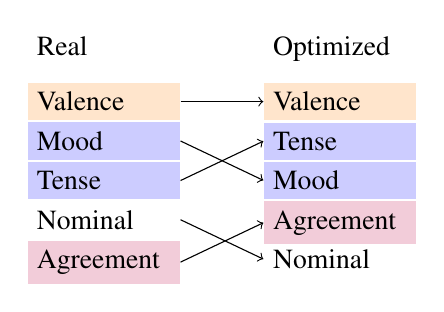
\begin{tikzpicture}[%
% common options for blocks:
block/.style = {draw, fill=blue!30, align=center, anchor=west,
            minimum height=0.65cm, inner sep=0},
% common options for the circles:
ball/.style = {circle, draw, align=center, anchor=north, inner sep=0}]
\node[rectangle,text width=1.7cm,anchor=base] (A0) at (1,-0.3) {Real};
\node[rectangle,text width=1.7cm,anchor=base] (B0) at (4,-0.3) {Optimized};
\node[rectangle,text width=1.7cm,anchor=base, fill=orange!20] (A1) at (1,-1.0) {Valence};
\node[rectangle,text width=1.7cm,anchor=base, fill=blue!20] (A2) at (1,-1.5) {Mood};
\node[rectangle,text width=1.7cm,anchor=base, fill=blue!20] (A3) at (1,-2.0) {Tense};
\node[rectangle,text width=1.7cm,anchor=base] (A4) at (1,-2.5) {Nominal};
\node[rectangle,text width=1.7cm,anchor=base, fill=purple!20] (A5) at (1,-3.0) {Agreement};
\node[rectangle,text width=1.7cm,anchor=base, fill=orange!20] (B1) at (4,-1.0) {Valence};
\node[rectangle,text width=1.7cm,anchor=base, fill=blue!20] (B2) at (4,-1.5) {Tense};
\node[rectangle,text width=1.7cm,anchor=base, fill=blue!20] (B3) at (4,-2.0) {Mood};
\node[rectangle,text width=1.7cm,anchor=base, fill=purple!20] (B4) at (4,-2.5) {Agreement};
\node[rectangle,text width=1.7cm,anchor=base] (B5) at (4,-3.0) {Nominal};
\draw[->] (A1.east) to (B1.west);
\draw[->] (A2.east) to (B3.west);
\draw[->] (A3.east) to (B2.west);
\draw[->] (A4.east) to (B5.west);
\draw[->] (A5.east) to (B4.west);
\end{tikzpicture}

  \end{minipage}
  &
    \begin{minipage}{.3\textwidth}
    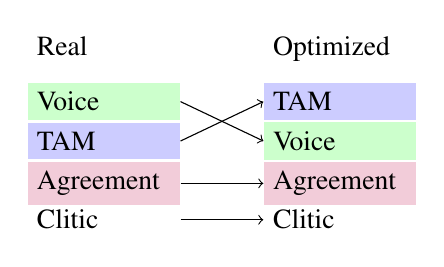
\begin{tikzpicture}[%
% common options for blocks:
block/.style = {draw, fill=blue!30, align=center, anchor=west,
            minimum height=0.65cm, inner sep=0},
% common options for the circles:
ball/.style = {circle, draw, align=center, anchor=north, inner sep=0}]
\node[rectangle,text width=1.7cm,anchor=base] (A0) at (1,-0.3) {Real};
\node[rectangle,text width=1.7cm,anchor=base] (B0) at (4,-0.3) {Optimized};
\node[rectangle,text width=1.7cm,anchor=base, fill=green!20] (A1) at (1,-1.0) {Voice};
\node[rectangle,text width=1.7cm,anchor=base, fill=blue!20] (A2) at (1,-1.5) {TAM};
\node[rectangle,text width=1.7cm,anchor=base, fill=purple!20] (A3) at (1,-2.0) {Agreement};
\node[rectangle,text width=1.7cm,anchor=base] (A4) at (1,-2.5) {Clitic};
\node[rectangle,text width=1.7cm,anchor=base, fill=blue!20] (B1) at (4,-1.0) {TAM};
\node[rectangle,text width=1.7cm,anchor=base, fill=green!20] (B2) at (4,-1.5) {Voice};
\node[rectangle,text width=1.7cm,anchor=base, fill=purple!20] (B3) at (4,-2.0) {Agreement};
\node[rectangle,text width=1.7cm,anchor=base] (B4) at (4,-2.5) {Clitic};
\draw[->] (A1.east) to (B2.west);
\draw[->] (A2.east) to (B1.west);
\draw[->] (A3.east) to (B3.west);
\draw[->] (A4.east) to (B4.west);
\end{tikzpicture}

  \end{minipage}
  \\
  \textsc{Korean}  & \textsc{Japanese} & \textsc{Sesotho Prefixes} \\
      \begin{minipage}{.3\textwidth}
    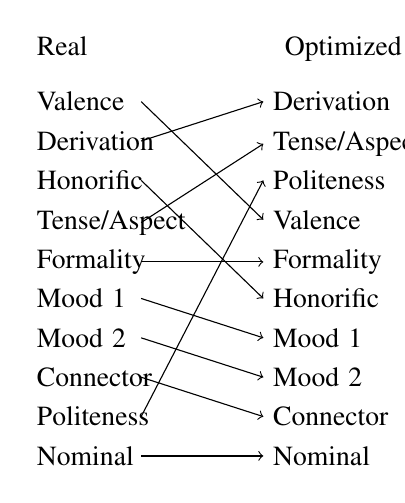
\begin{tikzpicture}[%
% common options for blocks:
block/.style = {draw, fill=blue!30, align=center, anchor=west,
            minimum height=0.65cm, inner sep=0},
% common options for the circles:
ball/.style = {circle, draw, align=center, anchor=north, inner sep=0}]
\node[rectangle,text width=1.2cm,anchor=base] (A0) at (1,-0.3) {Real};
\node[rectangle,text width=0.9cm,anchor=base] (B0) at (4,-0.3) {Optimized};
\node[rectangle,text width=1.2cm,anchor=base] (A1) at (1,-1.0) {Valence};
\node[rectangle,text width=1.2cm,anchor=base] (A2) at (1,-1.5) {Derivation};
\node[rectangle,text width=1.2cm,anchor=base] (A3) at (1,-2.0) {Honorific};
\node[rectangle,text width=1.2cm,anchor=base] (A4) at (1,-2.5) {Tense/Aspect};
\node[rectangle,text width=1.2cm,anchor=base] (A5) at (1,-3.0) {Formality};
\node[rectangle,text width=1.2cm,anchor=base] (A6) at (1,-3.5) {Mood 1};
\node[rectangle,text width=1.2cm,anchor=base] (A7) at (1,-4.0) {Mood 2};
\node[rectangle,text width=1.2cm,anchor=base] (A8) at (1,-4.5) {Connector};
\node[rectangle,text width=1.2cm,anchor=base] (A9) at (1,-5.0) {Politeness};
\node[rectangle,text width=1.2cm,anchor=base] (A10) at (1,-5.5) {Nominal};
\node[rectangle,text width=1.2cm,anchor=base] (B1) at (4,-1.0) {Derivation};
\node[rectangle,text width=1.2cm,anchor=base] (B2) at (4,-1.5) {Tense/Aspect};
\node[rectangle,text width=1.2cm,anchor=base] (B3) at (4,-2.0) {Politeness};
\node[rectangle,text width=1.2cm,anchor=base] (B4) at (4,-2.5) {Valence};
\node[rectangle,text width=1.2cm,anchor=base] (B5) at (4,-3.0) {Formality};
\node[rectangle,text width=1.2cm,anchor=base] (B6) at (4,-3.5) {Honorific};
\node[rectangle,text width=1.2cm,anchor=base] (B7) at (4,-4.0) {Mood 1};
\node[rectangle,text width=1.2cm,anchor=base] (B8) at (4,-4.5) {Mood 2};
\node[rectangle,text width=1.2cm,anchor=base] (B9) at (4,-5.0) {Connector};
\node[rectangle,text width=1.2cm,anchor=base] (B10) at (4,-5.5) {Nominal};
\draw[->] (A1.east) to (B4.west);
\draw[->] (A2.east) to (B1.west);
\draw[->] (A3.east) to (B6.west);
\draw[->] (A4.east) to (B2.west);
\draw[->] (A5.east) to (B5.west);
\draw[->] (A6.east) to (B7.west);
\draw[->] (A7.east) to (B8.west);
\draw[->] (A8.east) to (B9.west);
\draw[->] (A9.east) to (B3.west);
\draw[->] (A10.east) to (B10.west);
\end{tikzpicture}

  \end{minipage}
  &
  \begin{minipage}{.3\textwidth}
    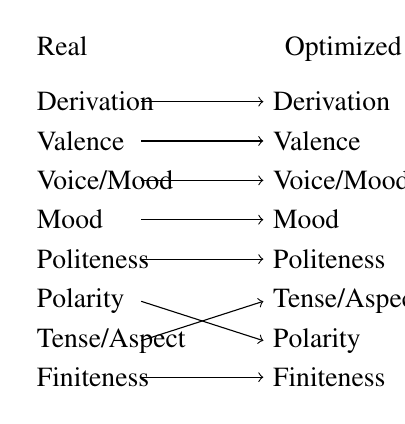
\begin{tikzpicture}[%
% common options for blocks:
block/.style = {draw, fill=blue!30, align=center, anchor=west,
            minimum height=0.65cm, inner sep=0},
% common options for the circles:
ball/.style = {circle, draw, align=center, anchor=north, inner sep=0}]
\node[rectangle,text width=1.2cm,anchor=base] (A0) at (1,-0.3) {Real};
\node[rectangle,text width=0.9cm,anchor=base] (B0) at (4,-0.3) {Optimized};
\node[rectangle,text width=1.2cm,anchor=base] (A1) at (1,-1.0) {Derivation};
\node[rectangle,text width=1.2cm,anchor=base] (A2) at (1,-1.5) {Valence};
\node[rectangle,text width=1.2cm,anchor=base] (A3) at (1,-2.0) {Voice/Mood};
\node[rectangle,text width=1.2cm,anchor=base] (A4) at (1,-2.5) {Mood};
\node[rectangle,text width=1.2cm,anchor=base] (A5) at (1,-3.0) {Politeness};
\node[rectangle,text width=1.2cm,anchor=base] (A6) at (1,-3.5) {Polarity};
\node[rectangle,text width=1.2cm,anchor=base] (A7) at (1,-4.0) {Tense/Aspect};
\node[rectangle,text width=1.2cm,anchor=base] (A8) at (1,-4.5) {Finiteness};
\node[rectangle,text width=1.2cm,anchor=base] (B1) at (4,-1.0) {Derivation};
\node[rectangle,text width=1.2cm,anchor=base] (B2) at (4,-1.5) {Valence};
\node[rectangle,text width=1.2cm,anchor=base] (B3) at (4,-2.0) {Voice/Mood};
\node[rectangle,text width=1.2cm,anchor=base] (B4) at (4,-2.5) {Mood};
\node[rectangle,text width=1.2cm,anchor=base] (B5) at (4,-3.0) {Politeness};
\node[rectangle,text width=1.2cm,anchor=base] (B6) at (4,-3.5) {Tense/Aspect};
\node[rectangle,text width=1.2cm,anchor=base] (B7) at (4,-4.0) {Polarity};
\node[rectangle,text width=1.2cm,anchor=base] (B8) at (4,-4.5) {Finiteness};
\draw[->] (A1.east) to (B1.west);
\draw[->] (A2.east) to (B2.west);
\draw[->] (A3.east) to (B3.west);
\draw[->] (A4.east) to (B4.west);
\draw[->] (A5.east) to (B5.west);
\draw[->] (A6.east) to (B7.west);
\draw[->] (A7.east) to (B6.west);
\draw[->] (A8.east) to (B8.west);
\end{tikzpicture}

  \end{minipage}
  &
  \begin{minipage}{.3\textwidth}
    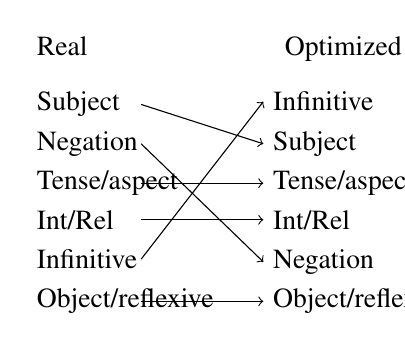
\begin{tikzpicture}[%
% common options for blocks:
block/.style = {draw, fill=blue!30, align=center, anchor=west,
            minimum height=0.65cm, inner sep=0},
% common options for the circles:
ball/.style = {circle, draw, align=center, anchor=north, inner sep=0}]
\node[rectangle,text width=1.2cm,anchor=base] (A0) at (1,-0.3) {Real};
\node[rectangle,text width=0.9cm,anchor=base] (B0) at (4,-0.3) {Optimized};
\node[rectangle,text width=1.2cm,anchor=base] (A1) at (1,-1.0) {Subject};
\node[rectangle,text width=1.2cm,anchor=base] (A2) at (1,-1.5) {Negation};
\node[rectangle,text width=1.2cm,anchor=base] (A3) at (1,-2.0) {Tense/aspect};
\node[rectangle,text width=1.2cm,anchor=base] (A4) at (1,-2.5) {Int/Rel};
\node[rectangle,text width=1.2cm,anchor=base] (A5) at (1,-3.0) {Infinitive};
\node[rectangle,text width=1.2cm,anchor=base] (A6) at (1,-3.5) {Object/reflexive};
\node[rectangle,text width=1.2cm,anchor=base] (B1) at (4,-1.0) {Infinitive};
\node[rectangle,text width=1.2cm,anchor=base] (B2) at (4,-1.5) {Subject};
\node[rectangle,text width=1.2cm,anchor=base] (B3) at (4,-2.0) {Tense/aspect};
\node[rectangle,text width=1.2cm,anchor=base] (B4) at (4,-2.5) {Int/Rel};
\node[rectangle,text width=1.2cm,anchor=base] (B5) at (4,-3.0) {Negation};
\node[rectangle,text width=1.2cm,anchor=base] (B6) at (4,-3.5) {Object/reflexive};
\draw[->] (A1.east) to (B2.west);
\draw[->] (A2.east) to (B5.west);
\draw[->] (A3.east) to (B3.west);
\draw[->] (A4.east) to (B4.west);
\draw[->] (A5.east) to (B1.west);
\draw[->] (A6.east) to (B6.west);
\end{tikzpicture}

  \end{minipage} \\
  \textsc{Sesotho Suffixes} \\
  \begin{minipage}{.3\textwidth}
    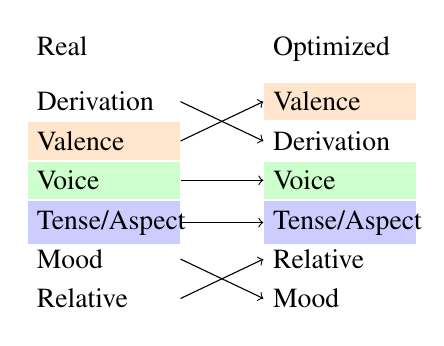
\begin{tikzpicture}[%
% common options for blocks:
block/.style = {draw, fill=blue!30, align=center, anchor=west,
            minimum height=0.65cm, inner sep=0},
% common options for the circles:
ball/.style = {circle, draw, align=center, anchor=north, inner sep=0}]
\node[rectangle,text width=1.7cm,anchor=base] (A0) at (1,-0.3) {Real};
\node[rectangle,text width=1.7cm,anchor=base] (B0) at (4,-0.3) {Optimized};
\node[rectangle,text width=1.7cm,anchor=base] (A1) at (1,-1.0) {Derivation};
\node[rectangle,text width=1.7cm,anchor=base, fill=orange!20] (A2) at (1,-1.5) {Valence};
\node[rectangle,text width=1.7cm,anchor=base, fill=green!20] (A3) at (1,-2.0) {Voice};
\node[rectangle,text width=1.7cm,anchor=base, fill=blue!20] (A4) at (1,-2.5) {Tense/Aspect};
\node[rectangle,text width=1.7cm,anchor=base] (A5) at (1,-3.0) {Mood};
\node[rectangle,text width=1.7cm,anchor=base] (A6) at (1,-3.5) {Relative};
\node[rectangle,text width=1.7cm,anchor=base, fill=orange!20] (B1) at (4,-1.0) {Valence};
\node[rectangle,text width=1.7cm,anchor=base] (B2) at (4,-1.5) {Derivation};
\node[rectangle,text width=1.7cm,anchor=base, fill=green!20] (B3) at (4,-2.0) {Voice};
\node[rectangle,text width=1.7cm,anchor=base, fill=blue!20] (B4) at (4,-2.5) {Tense/Aspect};
\node[rectangle,text width=1.7cm,anchor=base] (B5) at (4,-3.0) {Relative};
\node[rectangle,text width=1.7cm,anchor=base] (B6) at (4,-3.5) {Mood};
\draw[->] (A1.east) to (B2.west);
\draw[->] (A2.east) to (B1.west);
\draw[->] (A3.east) to (B3.west);
\draw[->] (A4.east) to (B4.west);
\draw[->] (A5.east) to (B6.west);
\draw[->] (A6.east) to (B5.west);
\end{tikzpicture}

  \end{minipage}
  \end{tabular}
  
  
    \caption{Real and optimized ordering (verbs)}
    \label{fig:real_and_optimized_verbs}
\end{figure}



\begin{figure}
\begin{tabular}{ccccccc}
\textsc{Finnish} & \textsc{Hungarian} & \textsc{Turkish} \\
\begin{minipage}{.3\textwidth}
    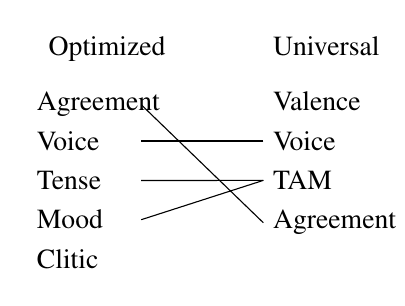
\begin{tikzpicture}[%
% common options for blocks:
block/.style = {draw, fill=blue!30, align=center, anchor=west,
            minimum height=0.65cm, inner sep=0},
% common options for the circles:
ball/.style = {circle, draw, align=center, anchor=north, inner sep=0}]
\node[rectangle,text width=1.2cm,anchor=base] (A0) at (4,-0.3) {Universal};
\node[rectangle,text width=0.9cm,anchor=base] (B0) at (1,-0.3) {Optimized};
\node[rectangle,text width=1.2cm,anchor=base] (A1) at (4,-1.0) {Valence};
\node[rectangle,text width=1.2cm,anchor=base] (A2) at (4,-1.5) {Voice};
\node[rectangle,text width=1.2cm,anchor=base] (A3) at (4,-2.0) {TAM};
\node[rectangle,text width=1.2cm,anchor=base] (A4) at (4,-2.5) {Agreement};
\node[rectangle,text width=1.2cm,anchor=base] (B1) at (1,-1.0) {Agreement};
\node[rectangle,text width=1.2cm,anchor=base] (B2) at (1,-1.5) {Voice};
\node[rectangle,text width=1.2cm,anchor=base] (B3) at (1,-2.0) {Tense};
\node[rectangle,text width=1.2cm,anchor=base] (B4) at (1,-2.5) {Mood};
\node[rectangle,text width=1.2cm,anchor=base] (B5) at (1,-3.0) {Clitic};
\draw[-] (A4.west) to (B1.east);
\draw[-] (A2.west) to (B2.east);
\draw[-] (A3.west) to (B3.east);
\draw[-] (A3.west) to (B4.east);
\end{tikzpicture}

    \end{minipage}
    &
    \begin{minipage}{.3\textwidth}
    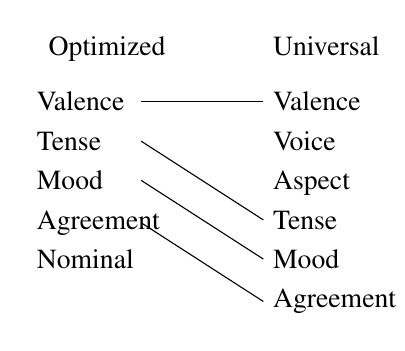
\begin{tikzpicture}[%
% common options for blocks:
block/.style = {draw, fill=blue!30, align=center, anchor=west,
            minimum height=0.65cm, inner sep=0},
% common options for the circles:
ball/.style = {circle, draw, align=center, anchor=north, inner sep=0}]
\node[rectangle,text width=1.2cm,anchor=base] (A0) at (4,-0.3) {Universal};
\node[rectangle,text width=0.9cm,anchor=base] (B0) at (1,-0.3) {Optimized};
\node[rectangle,text width=1.2cm,anchor=base] (A1) at (4,-1.0) {Valence};
\node[rectangle,text width=1.2cm,anchor=base] (A2) at (4,-1.5) {Voice};
\node[rectangle,text width=1.2cm,anchor=base] (A3) at (4,-2.0) {Aspect};
\node[rectangle,text width=1.2cm,anchor=base] (A4) at (4,-2.5) {Tense};
\node[rectangle,text width=1.2cm,anchor=base] (A5) at (4,-3.0) {Mood};
\node[rectangle,text width=1.2cm,anchor=base] (A6) at (4,-3.5) {Agreement};
\node[rectangle,text width=1.2cm,anchor=base] (B1) at (1,-1.0) {Valence};
\node[rectangle,text width=1.2cm,anchor=base] (B2) at (1,-1.5) {Tense};
\node[rectangle,text width=1.2cm,anchor=base] (B3) at (1,-2.0) {Mood};
\node[rectangle,text width=1.2cm,anchor=base] (B4) at (1,-2.5) {Agreement};
\node[rectangle,text width=1.2cm,anchor=base] (B5) at (1,-3.0) {Nominal};
\draw[-] (A1.west) to (B1.east);
\draw[-] (A4.west) to (B2.east);
\draw[-] (A5.west) to (B3.east);
\draw[-] (A6.west) to (B4.east);
\end{tikzpicture}

    \end{minipage}
        &
    \begin{minipage}{.3\textwidth}
    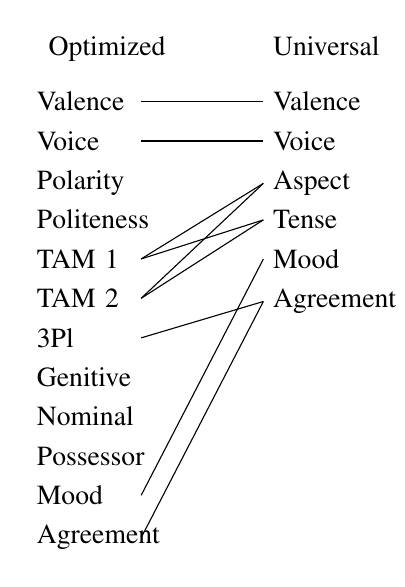
\begin{tikzpicture}[%
% common options for blocks:
block/.style = {draw, fill=blue!30, align=center, anchor=west,
            minimum height=0.65cm, inner sep=0},
% common options for the circles:
ball/.style = {circle, draw, align=center, anchor=north, inner sep=0}]
\node[rectangle,text width=1.2cm,anchor=base] (A0) at (4,-0.3) {Universal};
\node[rectangle,text width=0.9cm,anchor=base] (B0) at (1,-0.3) {Optimized};
\node[rectangle,text width=1.2cm,anchor=base] (A1) at (4,-1.0) {Valence};
\node[rectangle,text width=1.2cm,anchor=base] (A2) at (4,-1.5) {Voice};
\node[rectangle,text width=1.2cm,anchor=base] (A3) at (4,-2.0) {Aspect};
\node[rectangle,text width=1.2cm,anchor=base] (A4) at (4,-2.5) {Tense};
\node[rectangle,text width=1.2cm,anchor=base] (A5) at (4,-3.0) {Mood};
\node[rectangle,text width=1.2cm,anchor=base] (A6) at (4,-3.5) {Agreement};
\node[rectangle,text width=1.2cm,anchor=base] (B1) at (1,-1.0) {Valence};
\node[rectangle,text width=1.2cm,anchor=base] (B2) at (1,-1.5) {Voice};
\node[rectangle,text width=1.2cm,anchor=base] (B3) at (1,-2.0) {Polarity};
\node[rectangle,text width=1.2cm,anchor=base] (B4) at (1,-2.5) {Politeness};
\node[rectangle,text width=1.2cm,anchor=base] (B5) at (1,-3.0) {TAM 1};
\node[rectangle,text width=1.2cm,anchor=base] (B6) at (1,-3.5) {TAM 2};
\node[rectangle,text width=1.2cm,anchor=base] (B7) at (1,-4.0) {3Pl};
\node[rectangle,text width=1.2cm,anchor=base] (B8) at (1,-4.5) {Genitive};
\node[rectangle,text width=1.2cm,anchor=base] (B9) at (1,-5.0) {Nominal};
\node[rectangle,text width=1.2cm,anchor=base] (B10) at (1,-5.5) {Possessor};
\node[rectangle,text width=1.2cm,anchor=base] (B11) at (1,-6.0) {Mood};
\node[rectangle,text width=1.2cm,anchor=base] (B12) at (1,-6.5) {Agreement};
\draw[-] (A1.west) to (B1.east);
\draw[-] (A2.west) to (B2.east);
\draw[-] (A3.west) to (B5.east);
\draw[-] (A4.west) to (B5.east);
\draw[-] (A3.west) to (B6.east);
\draw[-] (A4.west) to (B6.east);
\draw[-] (A6.west) to (B7.east);
\draw[-] (A5.west) to (B11.east);
\draw[-] (A6.west) to (B12.east);
\end{tikzpicture}

    \end{minipage} 
    \\
    \textsc{Korean} & \textsc{Japanese} & \textsc{Sesotho Prefixes} \\
        \begin{minipage}{.3\textwidth}
    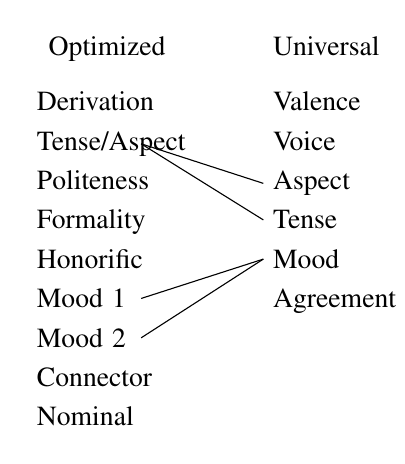
\begin{tikzpicture}[%
% common options for blocks:
block/.style = {draw, fill=blue!30, align=center, anchor=west,
            minimum height=0.65cm, inner sep=0},
% common options for the circles:
ball/.style = {circle, draw, align=center, anchor=north, inner sep=0}]
\node[rectangle,text width=1.2cm,anchor=base] (A0) at (4,-0.3) {Universal};
\node[rectangle,text width=0.9cm,anchor=base] (B0) at (1,-0.3) {Optimized};
\node[rectangle,text width=1.2cm,anchor=base] (A1) at (4,-1.0) {Valence};
\node[rectangle,text width=1.2cm,anchor=base] (A2) at (4,-1.5) {Voice};
\node[rectangle,text width=1.2cm,anchor=base] (A3) at (4,-2.0) {Aspect};
\node[rectangle,text width=1.2cm,anchor=base] (A4) at (4,-2.5) {Tense};
\node[rectangle,text width=1.2cm,anchor=base] (A5) at (4,-3.0) {Mood};
\node[rectangle,text width=1.2cm,anchor=base] (A6) at (4,-3.5) {Agreement};
\node[rectangle,text width=1.2cm,anchor=base] (B1) at (1,-1.0) {Derivation};
\node[rectangle,text width=1.2cm,anchor=base] (B2) at (1,-1.5) {Tense/Aspect};
\node[rectangle,text width=1.2cm,anchor=base] (B3) at (1,-2.0) {Politeness};
\node[rectangle,text width=1.2cm,anchor=base] (B4) at (1,-2.5) {Formality};
\node[rectangle,text width=1.2cm,anchor=base] (B5) at (1,-3.0) {Honorific};
\node[rectangle,text width=1.2cm,anchor=base] (B6) at (1,-3.5) {Mood 1};
\node[rectangle,text width=1.2cm,anchor=base] (B7) at (1,-4.0) {Mood 2};
\node[rectangle,text width=1.2cm,anchor=base] (B8) at (1,-4.5) {Connector};
\node[rectangle,text width=1.2cm,anchor=base] (B9) at (1,-5.0) {Nominal};
\draw[-] (A3.west) to (B2.east);
\draw[-] (A4.west) to (B2.east);
\draw[-] (A5.west) to (B6.east);
\draw[-] (A5.west) to (B7.east);
\end{tikzpicture}

    \end{minipage}
    &
    \begin{minipage}{.3\textwidth}
    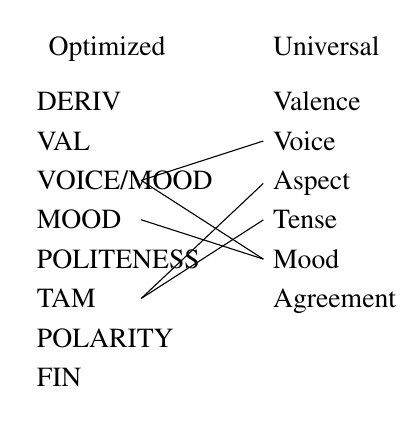
\begin{tikzpicture}[%
% common options for blocks:
block/.style = {draw, fill=blue!30, align=center, anchor=west,
            minimum height=0.65cm, inner sep=0},
% common options for the circles:
ball/.style = {circle, draw, align=center, anchor=north, inner sep=0}]
\node[rectangle,text width=1.2cm,anchor=base] (A0) at (4,-0.3) {Universal};
\node[rectangle,text width=0.9cm,anchor=base] (B0) at (1,-0.3) {Optimized};
\node[rectangle,text width=1.2cm,anchor=base] (A1) at (4,-1.0) {Valence};
\node[rectangle,text width=1.2cm,anchor=base] (A2) at (4,-1.5) {Voice};
\node[rectangle,text width=1.2cm,anchor=base] (A3) at (4,-2.0) {Aspect};
\node[rectangle,text width=1.2cm,anchor=base] (A4) at (4,-2.5) {Tense};
\node[rectangle,text width=1.2cm,anchor=base] (A5) at (4,-3.0) {Mood};
\node[rectangle,text width=1.2cm,anchor=base] (A6) at (4,-3.5) {Agreement};
\node[rectangle,text width=1.2cm,anchor=base] (B1) at (1,-1.0) {DERIV};
\node[rectangle,text width=1.2cm,anchor=base] (B2) at (1,-1.5) {VAL};
\node[rectangle,text width=1.2cm,anchor=base] (B3) at (1,-2.0) {VOICE/MOOD};
\node[rectangle,text width=1.2cm,anchor=base] (B4) at (1,-2.5) {MOOD};
\node[rectangle,text width=1.2cm,anchor=base] (B5) at (1,-3.0) {POLITENESS};
\node[rectangle,text width=1.2cm,anchor=base] (B6) at (1,-3.5) {TAM};
\node[rectangle,text width=1.2cm,anchor=base] (B7) at (1,-4.0) {POLARITY};
\node[rectangle,text width=1.2cm,anchor=base] (B8) at (1,-4.5) {FIN};
\draw[-] (A2.west) to (B3.east);
\draw[-] (A5.west) to (B3.east);
\draw[-] (A5.west) to (B4.east);
\draw[-] (A3.west) to (B6.east);
\draw[-] (A4.west) to (B6.east);
\end{tikzpicture}

    \end{minipage}
        &
    \begin{minipage}{.3\textwidth}
    \begin{tikzpicture}[%
% common options for blocks:
block/.style = {draw, fill=blue!30, align=center, anchor=west,
            minimum height=0.65cm, inner sep=0},
% common options for the circles:
ball/.style = {circle, draw, align=center, anchor=north, inner sep=0}]
\node[rectangle,text width=1.2cm,anchor=base] (A0) at (4,-0.3) {Universal};
\node[rectangle,text width=0.9cm,anchor=base] (B0) at (1,-0.3) {Optimized};
\node[rectangle,text width=1.2cm,anchor=base] (A1) at (4,-1.0) {Valence};
\node[rectangle,text width=1.2cm,anchor=base] (A2) at (4,-1.5) {Voice};
\node[rectangle,text width=1.2cm,anchor=base] (A3) at (4,-2.0) {Aspect};
\node[rectangle,text width=1.2cm,anchor=base] (A4) at (4,-2.5) {Tense};
\node[rectangle,text width=1.2cm,anchor=base] (A5) at (4,-3.0) {Mood};
\node[rectangle,text width=1.2cm,anchor=base] (A6) at (4,-3.5) {Agreement};
\node[rectangle,text width=1.2cm,anchor=base] (B1) at (1,-1.0) {Other_6};
\node[rectangle,text width=1.2cm,anchor=base] (B2) at (1,-1.5) {Other_2a};
\node[rectangle,text width=1.2cm,anchor=base] (B3) at (1,-2.0) {Infinitive};
\node[rectangle,text width=1.2cm,anchor=base] (B4) at (1,-2.5) {Other_ij};
\node[rectangle,text width=1.2cm,anchor=base] (B5) at (1,-3.0) {Other_wo};
\node[rectangle,text width=1.2cm,anchor=base] (B6) at (1,-3.5) {Other_di};
\node[rectangle,text width=1.2cm,anchor=base] (B7) at (1,-4.0) {Other_copula};
\node[rectangle,text width=1.2cm,anchor=base] (B8) at (1,-4.5) {Other_1s};
\node[rectangle,text width=1.2cm,anchor=base] (B9) at (1,-5.0) {Other_lo};
\node[rectangle,text width=1.2cm,anchor=base] (B10) at (1,-5.5) {Subject};
\node[rectangle,text width=1.2cm,anchor=base] (B11) at (1,-6.0) {Other_f^};
\node[rectangle,text width=1.2cm,anchor=base] (B12) at (1,-6.5) {Other_2};
\node[rectangle,text width=1.2cm,anchor=base] (B13) at (1,-7.0) {Tense/aspect};
\node[rectangle,text width=1.2cm,anchor=base] (B14) at (1,-7.5) {Int/Rel};
\node[rectangle,text width=1.2cm,anchor=base] (B15) at (1,-8.0) {Other_av};
\node[rectangle,text width=1.2cm,anchor=base] (B16) at (1,-8.5) {Negation};
\node[rectangle,text width=1.2cm,anchor=base] (B17) at (1,-9.0) {Other_9};
\node[rectangle,text width=1.2cm,anchor=base] (B18) at (1,-9.5) {Other_3};
\node[rectangle,text width=1.2cm,anchor=base] (B19) at (1,-10.0) {Other_17};
\node[rectangle,text width=1.2cm,anchor=base] (B20) at (1,-10.5) {Other_10};
\node[rectangle,text width=1.2cm,anchor=base] (B21) at (1,-11.0) {Other_7};
\node[rectangle,text width=1.2cm,anchor=base] (B22) at (1,-11.5) {Other_pr};
\node[rectangle,text width=1.2cm,anchor=base] (B23) at (1,-12.0) {Object/reflexive};
\draw[-] (A6.west) to (B10.east);
\draw[-] (A3.west) to (B13.east);
\draw[-] (A4.west) to (B13.east);
\draw[-] (A1.west) to (B23.east);
\end{tikzpicture}

    \end{minipage}
    \\
    \textsc{Sesotho Suffixes} \\
        \begin{minipage}{.3\textwidth}
    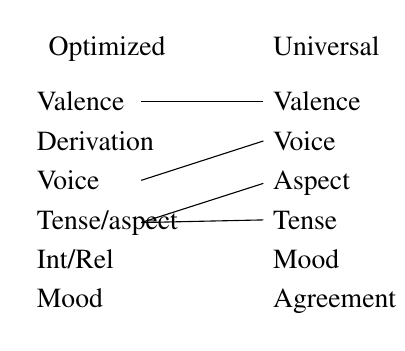
\begin{tikzpicture}[%
% common options for blocks:
block/.style = {draw, fill=blue!30, align=center, anchor=west,
            minimum height=0.65cm, inner sep=0},
% common options for the circles:
ball/.style = {circle, draw, align=center, anchor=north, inner sep=0}]
\node[rectangle,text width=1.2cm,anchor=base] (A0) at (4,-0.3) {Universal};
\node[rectangle,text width=0.9cm,anchor=base] (B0) at (1,-0.3) {Optimized};
\node[rectangle,text width=1.2cm,anchor=base] (A1) at (4,-1.0) {Valence};
\node[rectangle,text width=1.2cm,anchor=base] (A2) at (4,-1.5) {Voice};
\node[rectangle,text width=1.2cm,anchor=base] (A3) at (4,-2.0) {Aspect};
\node[rectangle,text width=1.2cm,anchor=base] (A4) at (4,-2.5) {Tense};
\node[rectangle,text width=1.2cm,anchor=base] (A5) at (4,-3.0) {Mood};
\node[rectangle,text width=1.2cm,anchor=base] (A6) at (4,-3.5) {Agreement};
\node[rectangle,text width=1.2cm,anchor=base] (B1) at (1,-1.0) {Valence};
\node[rectangle,text width=1.2cm,anchor=base] (B2) at (1,-1.5) {Derivation};
\node[rectangle,text width=1.2cm,anchor=base] (B3) at (1,-2.0) {Voice};
\node[rectangle,text width=1.2cm,anchor=base] (B4) at (1,-2.5) {Tense/aspect};
\node[rectangle,text width=1.2cm,anchor=base] (B5) at (1,-3.0) {Int/Rel};
\node[rectangle,text width=1.2cm,anchor=base] (B6) at (1,-3.5) {Mood};
\draw[-] (A1.west) to (B1.east);
\draw[-] (A2.west) to (B3.east);
\draw[-] (A3.west) to (B4.east);
\draw[-] (A4.west) to (B4.east);
\end{tikzpicture}

    \end{minipage}
\end{tabular}
    \caption{Comparing optimized orders with the universal order described by \citep{bybee-morphology-1985}.  Note that, for Sesotho prefixes, inversion of order relative to the universal order is expected, as the universal order indicates distance from the root, not absolute position.}
    \label{fig:optimized_and_universal_orders}
\end{figure}


\section{Discussion}

We have examined morpheme order in nouns and verbs in six morphologically rich and agglutinating languages, testing the recently propiosed Efficient Tradeoff Hypothesis \citep{hahn2020modeling} as an explanatory account of morpheme ordering.
We compared actual morpheme orderings to other possible orderings and to orderings optimized for efficiency of the memory-surprisal tradeoff.
In most cases, we found that the real ordering provided more efficient tradeoffs than most alternative orderings.
More importantly, we found that the real orderings match the optimal orderings in many respects.
Ordering forms found in a corpus according according to real or optimized orderings yields the same orders in XXX of cases.
In some cases, particularly for noun inflection, match between real and optimized orderings is perfect.
Beyond language-specific ordering patterns, optimization recovers previously-documented language universals of morpheme order.

\subsection{Relation to previous accounts}

%\subsubsection{Semantic Scope; Syntactic Structure; Historical Development}
%Morpheme ordering has been described from the perspective 
%Besides the explanation of broad typological tendencies, which we are interested in here, the linguistic literature has also debated at which level of linguistic representation morpheme ordering should be described, proposing accounts located at different levels such as the syntax-phonology interface \citep{baker1985the} and an autonomous layer of morphological description \citep{hyman2003suffix}.
%TODO also template vs scope vs...
%We do not see the memory--surprisal tradeoff as competing with or contradicting these studies.
%Rather, it specifies tendencies for ordering that could be implemented at different levels of linguistic description.

%\paragraph{Revelance and Proximity}


%A related family of explanations holds that those affixes are closest to the root that are most relevant to the root.
%Our optimized orders of Turkish and Hungarian \becky{Are there other languages?} perfectly match Bybee's proposed universal verbal inflection order (Figure REF).
%This suggests that high mutual information generally correlates with semantic relevance. 


In this section, we relate our results to existing explanatory accounts of morpheme ordering.


\cite{Hahn2020modeling} suggested that information locality provides a formalization of Bybee's \citep{bybee-morphology-1985} claim that semantic relevance determines ordering.
We suggest that mutual information provides an operational formalization of semantic relevance.
Relatedly, \citep{culbertson2020from} link conceptual closeness to MI, and argue that it is a driver of order (in the domain of noun phrase modifiers)

%TODO think about where to explain this As mentioned in section \becky{cite S2}, Bybee proposes a concept of \textit{semantic relevance}, which is the degree to which one morpheme affects the semantic content of the other \becky{cite bybee}. She hypothesizes that morphemes that are more highly relevant to each other should be closer to each other, and therefore proposes a universal ordering of verbal inflectional morphemes. For example, attaching a causative marker to a root meaning "to die" produces a verb form meaning "to kill." Since the causative greatly changes the semantic content of the original root, the causative is highly relevant to the root. 
%\becky{Format Korean example of juk-da ``to die" and juk-i-da ``to kill"}
%Bybee did not provide a way to computationally measure semantic relevance. 


%Other explanations suggest that morphemes are ordered based on (TODO CITE).
%The most straightforwardly related account is that of Bybee (1985) Semantic relevance
%CARP template in Bantu
%Explanations for the orders

%talk about Relevance and Mutual Information
%\paragraph{Morphemes as Fossilized Words}\
It has long been observed that the order of morphemes often parallels the order of independent words of corresponding meanings \citep{givon1971historical,venneman1973explanation,baker1985the}.
One explanation for this is that the order of morphemes reflects the order of formerly independent elements that have been fossilized into bound morphemes, which can often be verified in languages where historical data is available \citet{givon1971historical,venneman1973explanation}.
% interesting: Evans, Nicholas (1995). Multiple case in Kayardild: Anti-iconic suffix ordering and the diachronic filter. In Plank (ed.) 1995, 396-430. 
% Moravcsik, Edith A. (1995). Summing up Suffixaufnahme. In Plank (ed.) 1995, 451-484.  HEREL : 478, G24
% Cited by https://typo.uni-konstanz.de/rara/universals-archive/41/
On the other hand, \citet{bybee-morphology-1985} points out that there are historically documented cases where morpheme ordering has been restructured in ways that do not reflect former independent words, but respect the universal tendencies proposed by her (see also \citet{mithun2000the, haspelmath1993the, mithun1995affixation}; \citet[Section 15]{rice2000morpheme}).
A correspondence between the order of words and morphemes has also been postulated on a purely synchronic basis as a constraint on possible human languages.
For example, \cite{baker1985the} proposed the Mirror Principle, which -- informally -- states that the order of elements (morphemes) in morphology reflects the order of elements (words) in syntax.
A large body of work in theoretical syntax describes word and morpheme order using the same processes and principles \citep{halle1993distributed}.
As a theory of order at multiple levels, the Efficient Tradeoff Hypothesis is compatible with these different historical paths and predicts these ordering patterns independently of the historical path leading to the morphemes found in a given language.



%As the memory-surprisal tradeoff is optimized by word order, this is compatible with our results:
%To the extent that morpheme order does reflect fossilized word order, morpheme order should continue to reflect optimization for the tradeoff.


%To the extent that similar statistical patterns of usage hold for corresponding words and morphemes, this again is compatible with the Efficient Tradeoff Hypothesis.

%\mhahn{TODO regarding scope: \citep{baker1988incorporation,foley1984functional,chierchia1990meaning,valin1992a}}


%This can be related to the scope-based explanation to the extent that syntactic structure and word order reflect scope.
% INTERESTING reference: http://www.jzeller.de/pdf/CARP.pdf

%\paragraph{Semantic Scope}


%Description in terms of scope faces limitations when order is different from semantic scope.
%\cite{Hyman2003}
%Hyman  (2003:  249) proposed the CARP template to describe suffix order in Bantu languages (such as Sesotho), a templatic order for valence and voice morphemes that can be different from scope order.
%In \cite{Hyman2003}'s model, order is determined based on both the CARP template and a preference for ismorphism with semantic scope.
%

Another prominent account is in terms of semantic scope \citep{rice2000morpheme}.
This is the idea that morphemes are ordered in the order in which their meanings combine.
The relative ordering of valence and voice is a good example for the scope-based explanation.
Valence affixes change the number of arguments, and passive (voice) promotes one argument to the subject position.
This can affect an argument introduced by a voice marker.
The following example from Turkish illustrates this (\cite{schaaik2020turkish}, section 30.8.2):


\begin{tabular}{ccccccc}
don-dur-ul & freeze-caus-pass & be frozen \\
don-dur & freeze-caus & to freeze (something) \\
don & freeze& to freeze \\
\end{tabular}

Turkish has suffixes both for causative and passive.
When adding both suffixes simultaneously, the causative marker appears closer to the root.
This corresponds to the order in which the meanings of these suffixes combine with the meaning of the root:
Causative adds an argument indicating who makes an object freeze, and passive then removes that argument, yielding a verb describing something that is being frozen by someone.

A priori, semantic scope is different from mutual information.
However, there are arguments that scope relations correlate with mutual information.
\citet{culbertson2020from} made a related argument for the order of nominal modifiers as in ``the four green books'', where mutual information predicts the order of attachment of modifiers to the noun.
Furthermore, if the semantic propositions that speakers communicate are modeled using a probabilistic language of thought grammar such as CITE, mutual information will also correlate with scope ordering (see SI Appendix Section X for a simulation study).


%\paragraph{Templates}
%CARP template
%\cite{muysken1981quechua}
%\cite{mccarthy2008generalized} phonology
%\cite{hyman2003suffix}
%\cite{kanu2009suffix} morphotactics, not semantic scope







\subsection{Other Aspects of Morphology}

Our study focused on agglutination, where a word carries multiple clearly separated morphemes with distinct functions.
There are other types of morphological processes that deserve study.

Many languages show fusion where different categories are fused into a single morpheme, or stem changes, such as English swim $\rightarrow$ swam.
An extreme case is non-concatenative morphology (in Arabic, k-t-b `to write' forms katab- `wrote'. -aktub `write/be writing', -kutib- `was written').
These types of morphological processes are not described in terms of the order of different morphemes.


While we have focused on the relative distance from the root, we have not touched on the question of why a morpheme is realized as a prefix or a suffix in a given language.
There are well-known correlations between suffixing or prefixing preference and word order \citep{greenberg1963universals}.




\subsection{Limitations}

- genre of data: written. but Sesotho is spoken (child-directed)

- limitations of computational estimation of the memory-surprisal tradeoff. %However: As the set of all moprphological forms of a language is typically finite (CITE), we believe that these limitations play a smaller role in morpheme order, compared to word order.


A further limitation relates to the selection of languages.
The six languages considered in this study are spoken in Eurasia and Africa, not representing Australia and America.
Among the languages, Hungarian and Finnish are genetically related (X millenia).
There is also some evidence for genetic relations beyond these (Japanese, Korean, Turkish), but such relations would have to be quite ancient (x millenia).
The morphemes found in these languages as considered here are generally not cognate.
Thus, the commonalities in languages found cannot be traced to inherited orderings of morphemes inherited from a common ancestor.
Furthermore, we note that the optimality of different orderings crucially depend not on the morphemes themselves (which might be inherited), but on the frequencies of different forms (e.g., of sinulars and plurals).



\section{Conclusion}

We have tested the recently proposed Efficient Tradeoff Hypothesis as a predictor of morpheme order with data from verbs and nouns across six languages.
We found that attested morpheme orders provide more efficient tradeoffs than most other possible orderings and that many properties of observed orderings are recovered by optimizing for tradeoff efficiency.
With the exception of verb inflection in Finnish and Sesotho, we found that optimized orderings agree with the attested orderings in more than 90\% of forms found in corpora.
Optimization also successfully predicts several universals of morpheme ordering, both for nouns and verbs.


\bibliography{literature}
\bibliographystyle{natbib}


\end{document}

\appendix

\section{Appendix}

\tableofcontents

\section{Estimating Memory--Surprisal Tradeoffs and Constructing Optimized Orderings}


\section{Identifying Morphemes from Corpus Data}


In order to create these morpheme orderings, we first need to identify and label morphemes for each language. The Korean, Japanese, and Sesotho corpora have words segmented into the grapheme representations of their morphemes. However, the Turkish, Hungarian, and Finnish corpora do not segment the words into morphemes, but rather include a list of features (such as person, number, voice, etc.) present in each word. We built segmenters to reconstruct the order of morphemes in each word from those feature labels. See SI Appendix Section X for details.


 Grapheme, label, phoneme for Korean \mhahn{For now, I think we can place grapheme and phoneme versions into the appendix, and only discuss the MorphemeMeanings-based one in the main paper (i.e., ordering based on morpheme meanings, surprisal based on abstract morphemes, analogous to the Coarse+FineSurprisal version for the other languages.}
    The Korean corpus came with segmented morphemes labeled with fine-grained categories such as "ending final marker," or "predicative maker," which were the labels we used for the specific morpheme meaning segmenter. We also built a segmenter to take in each segment and output the abstract morpheme slot it fills (such as ``formality"), similar to the abstract slot labelling we did with Turkish, Hungarian, and Finnish. 

 \mhahn{In the main paper, I think it's enough to present the Coarse+FinalSurprisal results. We can present others in the appendix, and don't need to introduce them here in detail.} %We built two different segmenters for each of the Turkish, Hungarian, and Finnish corpora. One version was ``coarse-grained," meaning that we recovered the order of suffixes in the word on an abstract level, such as a list of ``subject person, subject number." The other version was ``fine-grained," meaning that we used more specific labels for each suffix, such as ``2nd person, plural." In the models, each word is represented as its list of coarse-grained labels, and the model tries to predict the fine-grained labels based on the coarse-grained abstract morphemes. As such, the model tries to order the fine-grained labels, but the surprisal is calculated on the basis of the coarse-grained abstract morphemes.
    
%    We built segmenters on two different levels of abstraction for the Finnish, Hungarian, and Turkish corpora. The more fine-grained segmenter version takes the list of morphological features present in a particular word and reconstructs the natural order of morphemes, labelling each morpheme with its specific meaning, such as ``2nd person plural subject." The more abstract segmenter takes the list of morphological features for each word and reconstructs the filled abstract morpheme slots for that word, where each slot has generic label such as ``agreement." For example, in Hungarian, the only possible slots of suffixes appearing after a verb root are voice, mood, tense, agreement, and clitics. As such, we can assign each slot an integer representing the order in which the slots can be filled in a certain language. 

\subsection{Korean Verb Suffixes}

Korean verb morphology is very complex, and there is no generally agreed-upon description in terms of morphemes and slots.
We extracted suffixes based on the annotation found in the Kaist corpus \citep{chun2018building} and the linguistic literature on Korean \citep{yeon2010korean}.
The Kaist corpus already provides segmentation into morphemes; we postprocessed it in two ways:
First, we made it more fine-grained by splitting morphemes that are merged in the annotation, and, second, we abstracted away consistently from allomorphy.
For instance, the Kaist corpus separately labels the segments \korean{ㅂ니다} \textit{-mnida} (as in \korean{합니다} \textit{hamnida} `does') and \korean{습니다} \textit{-seumnida} (as in \korean{했습니다} \textit{hatseumnida} `did').
These two segments actually are allomorphs, conditioned by the preceding material.
Furthermore, they can both be segmented into the formal marker \korean{ㅂ/습} (\textit{-p/-seup}, we label this underlying morpheme ``\textsc{p}$_5$'', see below for this notation), and the mood markers \korean{니} (\textit{-ni}, our \textsc{ni}$_6$) and \korean{다} (\textit{-da}, our \textsc{da}$_7$).
We therefore transform both segments into the abstract morpheme sequence \textsc{p}$_5$-\textsc{ni}$_6$-\textsc{da}$_7$ (see below for this notation).
We then partitioned the resulting morphemes into slots that make it possible to consistently describe the ordering of almost all forms encountered in the corpus.


With this procedure, we identified the nine slots described below:
\begin{enumerate}
    \item Root
    %. The root may include a valency suffix, which is not separated frem the root in the dataset. We did not attempt to separate v
    \item Derivation: The two derivational suffixes are \textit{ha} (\citep[4.1.2]{yeon2010korean}) and the predicative \textit{i}, whose function is similar to that of a copula \citep[4.1.4]{yeon2010korean}.
    
    \item Honorific \textsc{si}$_3$ \citep[4.3.2, 4.4.1]{yeon2010korean}
    \item Tense/Aspect suffixes include -\textsc{ess}$_4$ for past \citep[4.5.1.1]{yeon2010korean}, -\textsc{essess}$_4$ for remote past \citep[4.5.1.2]{yeon2010korean}, -\textsc{get}$_4$ for future \citep[4.5.2.1]{yeon2010korean}
    \item Formality \textsc{p}$_5$ (allomorphs include -\textit{p}-, -\textit{m}-, -\textit{seum}-,  \citep[4.3.2]{yeon2010korean})
    \item Mood 1: We partition Mood suffixes into two slots, as these can be combined into strings of combined mood suffixes. Frequent elements of the Mood I slot are -\textsc{n}$_6$-, -\textsc{ni}$_6$- \citep[4.3.2]{yeon2010korean}.
    
    \item Mood II: Frequent elements of the Mood II slot are declarative -\textsc{da}$_7$- \citep[4.3.2]{yeon2010korean}, command -\textsc{ra}-, interrogative -\textsc{ka}-, the suffix  -\textsc{ji} \citep[4.2.2-3]{yeon2010korean}, and informal -\textsc{eo}$_7$-.
    
    \item Polite -yo
    \item Conjunctive endings, such as -go, -seo,  and others
    
\end{enumerate}

We show morphemes occurring at least 50 times in slots 2-8 in Figure~\ref{tab:korean-frequent-morphemes}.
We do not provide the list of conjunctive and nominalizing suffixes since these are very numerous.

Additional morphemes that occur less than TODO times are placed into an UNKNOWN slot, this affects TODO \% of morpheme occurrences in the dataset.
We indicate morphemes by a small-caps representation of a stylized phonological representation (such as \textsc{p} for -\korean{ㅂ/습}  -\textit{p/seup}),\footnote{These transcriptions are purely conventional, we do not intend these to correspond to a theory of how underlying phonological forms are realized as surface phone strings.} with a subscript indicating their slot (such as \textsc{p}$_5$-\textsc{ni}$_6$-\textsc{da}$_7$).


%TODO 
%- Yeon 4.4.2.2 kkeo object honorific % 꺼   % does not seem to appear in Kaist corpus?


%Frequent morphemes:
\begin{table}
\resizebox{1.2\textwidth}{!}{
\begin{tabular}{llllllllll}
Slot & Morphs & Short & Freq. & Description & Citation \\ \hline\hline
Derivation & \korean{하} & HA$_2$ &	 68 & & \citep[4.1.2]{yeon2010korean}\\
& i & I$_2$ &	 3947 && \citep[4.1.4]{yeon2010korean} \\ \hline
Honorific & si 	& \textsc{si}$_3$ & 99 & &\citep[4.3.2, 4.4.1]{yeon2010korean}\\\hline
Tense/Asp. & \korean{었었} 	& ESSESS$_4$ &  56&& \citep[4.5.1.2]{yeon2010korean} \\
&get 	& GET$_4$ & 355 & assertive & \citep[4.5.2.1]{yeon2010korean}\\
& &ESS$_4$ &	 9720 & past& \citep[4.5.1.1]{yeon2010korean}\\\hline
Formality & p &P$_5$ &	 1761 & formal-polite &\citep[4.3.2]{yeon2010korean}\\\hline
Mood 1&ri & RI$_6$ &	 70 & I-guess-\\
&ni 	&NI$_6$ & 1700 && \citep[4.3.2]{yeon2010korean}\\
&n 	&N$_6$ &5069 & TODO  \\\hline
Mood 2&sida & SIDA$_7$ & 	 51 & Hortative, formal, polite \\
& \korean{어} 	& EO$_7$ & 62 & Indicative, informal\\
& \korean{자} & JA$_7$&	 163 & Hortative, formal, nonpolite & \citep[4.3.6.3]{yeon2010korean}\\
& \korean{소} &SO$_7$  &	 194 & See Table~\ref{tab:korean-styles} \\
& lkka & LKKA$_7$&	 200 & Interrogative & \citep[8.9]{yeon2010korean} \\
& \korean{오} & O$_7$ &	 226 & See Table~\ref{tab:korean-styles} \\
& ji & JI$_7$ &	 260 &    & \citep[4.2.2-3]{yeon2010korean}\\
& ka 	& KA$_7$ & 485 & Interrogative & \citep[4.3.4, p. 175; p. 183]{yeon2010korean} \\
& ra &RA$_7$ \korean{라} &	 959 & plain style command & \citep[4.3.6.4]{yeon2010korean} \\
& da & DA$_7$ &	 23035 & Declarative & \citep[4.3.2]{yeon2010korean} &  \\\hline
Polite & \korean{요} & YO$_8$&	 267 & See Table~\ref{tab:korean-styles} \\
\end{tabular}
}
\caption{Frequent Korean verb suffixes in slots 1-8.}\label{tab:korean-frequent-morphemes}
\end{table}


Next, we explain how our segmentation corresponds to commonly described paradigms.
First, in Table~\ref{tab:korean-styles}, we describe the correspondence to the speech style system described by \citep[4.3.2]{yeon2010korean}.
Second, in Tables~\ref{tab:korean-hada-1}--\ref{tab:korean-hada-3}, we show the paradigm for the verb \korean{하다} \textit{hada} `to do' as described in Wiktionary.\footnote{ \texttt{https://en.wiktionary.org/wiki/\korean{하다}} (retrieved Septemgber 16, 2020).}
In Table~\ref{tab:kroean-itda}, we show the part of the paradigm of the verb \textit{ida} `to be' corresponding to Table~\ref{tab:korean-hada-1} (the other parts of the paradigm are analogous to those of \textit{hada}).
Note that none of these paradigms constitute exhaustive lists of all forms of these verbs; instead, they represent commonly used forms in a systematic paradigmatic representation.


\begin{table}
	\begin{center}
\begin{tabular}{l||l|l|l|llll}
            & Statement & Question  & Command    & Proposal    \\ \hline\hline
Formal      &  \korean{ㅂ니다} & \korean{ㅂ니까} & \korean{지-ㅂ-지오} & \korean{지-ㅂ-지다} \\ 
      &  -mnida & -mnikka  & -sipsio & -sipsida  \\ 
      &  -\textsc{p}$_5$-\textsc{ni}$_6$-\textsc{da}$_7$ & -\textsc{p}$_5$-\textsc{ni}$_6$-\textsc{kka}$_7$  & -\textsc{si}$_3$-\textsc{p}$_5$-\textsc{sio}$_7$ & -\textsc{si}$_3$-\textsc{p}$_5$-\textsc{sida}$_7$ \\ \hline
Polite      &  \multicolumn{4}{c}{\korean{아/어/요}}  \\
      &  \multicolumn{4}{c}{-a/eoyo}  \\
            & \multicolumn{4}{c}{-\textsc{eo}$_7$-\textsc{yo}$_8$} \\ \hline
Semi-Formal & \korean{오/소}   &           &   \korean{오}       &  \korean{-ㅂ-지다} \\
&  -o/so   &           & -o        & -p-sida \\
 &  -O$_7$/-SO$_7$   &           & -O$_7$    & -\textsc{p}$_5$-\textsc{sida}$_7$ \\\hline
Familiar    &    \korean{네}    &  \korean{나/는가} &  \korean{게}      &    \korean{세} \\
            & -ne                  & -na/neunka & -ge & -se \\ 
            & -\textsc{ne}$_7$                  & -\textsc{na}$_7$/-\textsc{neunka}$_7$ & -GE$_9$ & \textcolor{red}{-SE} \\ \hline
Intimate      &  \multicolumn{4}{c}{\korean{아/어}}  \\
      &  \multicolumn{4}{c}{-a/eo}  \\
            & \multicolumn{4}{c}{-\textsc{eo}$_7$} \\ \hline
Plain       &   \korean{다}     &  \korean{(느)냐} &  \korean{라}     &  \korean{자}\\
            &  -da    &  -(neu)nya & -ra      & -ja \\
            & -\textsc{da}$_7$    &   -\textsc{nya}$_7$          & -RA$_7$      & -JA$_7$\\
\end{tabular}
	\end{center}
\caption{Correspondence between our morpheme segmentation and the speech style system described by \citep[4.3.2]{yeon2010korean}. In each cell, we provide the Hangul ending given by \citep{yeon2010korean}, a transliteration, and a representation in terms of underlying morphemes.}\label{tab:korean-styles}
\end{table}



\begin{table}
\begin{tabular}{llllllllll}
           &          &Formal non-polite & Informal non-polite & Informal polite & Formal polite \\ \hline \hline
\multirow{6}{*}{Indicative} & \multirow{3}{*}{Non-past} & \korean{한다} & \korean{해}  & \korean{해요}  & \korean{합니다}  \\
           &          & handa & hae & haeyo &  hamnida \\
           &          & -\textsc{n}$_6$-\textsc{da}$_7$ & -\textsc{eo}$_7$ & -\textsc{eo}$_7$-\textsc{yo}$_8$ &  -\textsc{p}$_5$-\textsc{ni}$_6$-\textsc{da}$_7$ \\
           &          & \korean{하+ㄴ다}  & \korean{하+어}    & \korean{하+어+요} & \korean{하+ㅂ니다} \\
            &          &  px+ef        &   pvg+ecs        & pvg+ef+jxf & pvg+ef\\
           \hline
           & \multirow{3}{*}{Past}     & \korean{했다}  & \korean{했어} & \korean{했어요}   & \korean{했습니다}  \\
           &      & haet-da &  haesseo &  haesseoyo  & haetseumnida \\
           &      & -\textsc{ess}$_4$-\textsc{da}$_7$ &  -\textsc{ess}$_4$-\textsc{eo}$_7$ &  -\textsc{ess}$_4$-\textsc{eo}$_7$-\textsc{yo}$_8$  & -\textsc{ess}$_4$-\textsc{p}$_5$-\textsc{ni}$_6$-\textsc{da}$_7$ \\
           &      &  \korean{하+었+다}  &  \korean{하+었+어} & \korean{하+었+어+요} & \korean{하+었+습니다}  \\
           &      &  ncpa+xsv+ep+ef   & px+ep+ef   &   px+ep+ef+jxf &     pvg+ep+ef\\
           \hline
\multirow{6}{*}{Interrogative} & \multirow{3}{*}{Non-past} & \korean{하느냐} & \korean{해}  & \korean{해요}  & \korean{합니까} \\
 &  & haneunya &  hae &  haeyo & hamnikka\\
 &  & -\textsc{nya}$_7$ &  -\textsc{eo}$_7$ &  -\textsc{eo}$_7$-\textsc{yo}$_8$ & -\textsc{p}$_5$-\textsc{ni}$_6$+KKA$_7$ \\
               && \korean{하+느냐} & & & \korean{하+ㅂ니까}    \\
              && px+ef & & & px+ef \\
 \hline
              & \multirow{3}{*}{Past} & \korean{했느냐} & \korean{했어} & \korean{했어요} & \korean{했습니까} \\
              &  & ha-n-neunya &  hae-sseo &  hae-sseo-yo &  haetseumnikka\\
              &  & -\textsc{ess}$_4$-\textsc{nya}$_7$ &  -\textsc{ess}$_4$-\textsc{eo}$_7$ &  -\textsc{ess}$_4$-\textsc{eo}$_7$+YO$_8$ &  -\textsc{ess}$_4$-\textsc{p}$_5$-\textsc{ni}$_6$-\textsc{kka}$_7$\\
              &  &  \korean{하+었+느냐}  & \korean{하+었+어} & \korean{하+었+어+요} & \korean{하+었+습니까} \\
              &  & +ep+ef  & +ep+ef            & px+ep+ef+jxf & pvg+ep+ef \\
              \hline
Hortative   && \korean{하자}  & \korean{해}  & \korean{해요}  & \korean{합시다}  \\
   && haja &  hae &  haeyo & hapsida \\
   && -JA$_7$ &  -\textsc{eo}$_7$ &  -\textsc{eo}$_7$-\textsc{yo}$_8$ & -\textsc{p}$_5$-\textsc{sida}$_7$ \\
   && \korean{+자} && \korean{하+어+요} & \korean{하+ㅂ시다}\\
   && +ef  && pvg+ef+jxf & ef \\
   \hline
Imperative  && \korean{해라, 하여라}  & \korean{해}  & \korean{해요}  & \korean{합시오}  \\
  && haera, hayeora &  hae &  haeyo &  hapsio \\
  && -\textsc{ra}$_7$ & -\textsc{eo}$_7$ & -\textsc{eo}$_7$-\textsc{yo}$_8$ & -\textsc{p}$_5$-\textsc{si}$_3$O \\
  && \korean{하+어라}, \korean{하+어라}  &  &    & \korean{+ㅂ시오} \\
  && pvg+ef,  pvg+ef                     &  &    &  +ef\\
  \hline
Assertive   && \korean{하겠다}  & \korean{하겠어}  & \korean{하겠어요}  & \korean{하겠습니다}  \\
   &&  hagetda & hagesseo &  hagesseoyo & hagetseumnida \\
   &&  -\textsc{get}$_4$-\textsc{da}$_7$ & -\textsc{get}$_4$-\textsc{eo}$_7$ &  -\textsc{get}$_4$-\textsc{eo}$_7$-\textsc{yo}$_8$ & \textsc{get}$_4$-\textsc{p}$_5$-\textsc{ni}$_6$-\textsc{da}$_7$ \\
&& \korean{하+겠+다}  & \korean{하+겠+어}   & \korean{하+겠+어+요} & \korean{하+겠+습니다}\\
&&  px+ep+ef          & pvg+ep+ef   & pvg+ep+ef+jxf & pvg+ep+ef\\
\hline
\end{tabular}
	\caption{Correspondence between our morpheme segmentation and the paradigm of \textit{hada} `to do' as described by Wiktionary and in the Kaist treebank. In each cell, we provide the Hangul  and transliterated (e.g., handa) forms given by Wiktionary, a representation in terms of underlying morphemes (e.g., -\textsc{n}$_6$-\textsc{da}$_7$), and -- where available -- how the form is segmented in the Kaist corpus (e.g., px+ef).}\label{tab:korean-hada-1} % (e.g., \korean{한다})\korean{하+ㄴ다} and 
\end{table}

\begin{table}
	\begin{center}
\begin{tabular}{llllllllll}
           &          &Formal non-polite & Informal non-polite & Informal polite & Formal polite \\ \hline \hline
Cause/Reason && \korean{해} & \korean{해서, 하여서} & \korean{하니} & \korean{하니까} \\
&& hae & haeseo, hayeoseo & hani & hanikka \\ 
&& -\textsc{eo}$_7$ & -\textsc{eoseo}$_9$ & -\textsc{ni}$_9$ & -\textsc{nikka}$_9$ \\
&& &\korean{하+어서, 하+어서} & \korean{하+니} & \korean{하+니까} \\
&& & pvg+ecs, xsm+ecs         & pvg+ecs & xsm+ef \\
\hline
Contrast && \korean{하지만} & \korean{하는데} & \korean{하더니} \\
 && hajiman & haneunde & haedoni & \\ 
 && -\textsc{jiman}$_9$ & -\textsc{neunde}$_9$ & -\textsc{deoni}$_9$ & \\ \hline
Conjunction && \korean{하고} \\
 && hago \\ 
	&& -\textsc{go}$_9$ \\ \hline
Condition && \korean{하면} & \korean{해야, 하여야} \\
&& hamyeon & haeya, hayeoya \\
	&& -\textsc{meyon}$_9$ & -\textsc{eoya}$_9$ \\ \hline
Motive && \korean{하려고} \\
 && haryeogo \\
&& -RYEOGO$_9$
\end{tabular}
	\end{center}
	\caption{Continuation of Table~\ref{tab:korean-hada-1}: Forms of \textit{hada} with a conjunctive ending.}\label{tab:korean-hada-2}
\end{table}



\begin{table}[]
    \centering
    \begin{tabular}{llllllllllllllllllllllllll}
           &          &Formal non-polite & Informal non-polite & Informal polite & Formal polite \\ \hline \hline
\multirow{2}{*}{Indicative} & Non-past & \korean{하신다} & \korean{하셔} & \korean{하세요, 하셔요} & \korean{하십니다} \\
                           && -\textsc{si}$_3$-\textsc{n}$_6$-\textsc{da}$_7$ & \textsc{si}$_3$-\textsc{eo}$_7$ & \textsc{si}$_3$-\textsc{eo}$_7$-\textsc{yo} & \textsc{si}$_3$-\textsc{p}$_5$-\textsc{ni}$_6$-\textsc{da}$_7$ \\
&& \korean{하+시+ㄴ다}       &   --   &    \korean{하+시+어+요}             &  \korean{하+시+ㅂ니다}        \\
\hline
&& \korean{하셨다} & \korean{하셨어} & \korean{하셨어요} & \korean{하셨습니다} \\
&& \textsc{si}$_3$-\textsc{ess}$_4$-\textsc{da}$_7$ & \textsc{si}$_3$-\textsc{ess}$_4$-\textsc{eo}$_7$ & \textsc{si}$_3$-\textsc{ess}$_4$-\textsc{eo}$_7$-\textsc{yo} & \textsc{si}$_3$-\textsc{ess}$_4$-\textsc{p}$_5$-\textsc{ni}$_6$-\textsc{da}$_7$ \\
& & \korean{하+셨+다}       &  --    &        --        &  \korean{하+셨+습니다}       \\
\hline
\multirow{2}{*}{Interrogative} & Non-past & \korean{하시느냐} & \korean{하셔} & \korean{하세요, 하셔요} & \korean{하십니까} \\
&& \textsc{si}$_3$-\textsc{nya}$_7$ & \textsc{si}$_3$-\textsc{eo}$_7$ & \textsc{si}$_3$-\textsc{eo}$_7$-\textsc{yo} & \textsc{si}$_3$-\textsc{p}$_5$-\textsc{ni}$_6$-\textsc{kka}$_7$ \\
& &   --     &   --   &   \korean{하+시+어+요}             &  --        \\
\hline
& Past & \korean{하셨느냐} & \korean{하셨어} & \korean{하셨어요} & \korean{하셨습니까} \\
&      & \textsc{si}$_3$-\textsc{ess}$_4$-\textsc{nya}$_7$ & \textsc{si}$_3$-\textsc{ess}$_4$-\textsc{eo}$_7$          & \textsc{si}$_3$-\textsc{ess}$_4$-\textsc{eo}$_7$-\textsc{yo} & \textsc{si}$_3$-\textsc{ess}$_4$-\textsc{p}$_5$-\textsc{ni}$_6$-\textsc{kka}$_7$ \\
& &        &      &                &          \\
\hline
\multirow{2}{*}{Imperative} && \korean{하시라} & \korean{하셔} & \korean{하세요} & \korean{하십시오} \\
&& -\textsc{si}$_3$-RA & -\textsc{si}$_3$-\textsc{eo}$_7$ & -\textsc{si}$_3$-\textsc{eo}$_7$-\textsc{yo} & -\textsc{si}$_3$-\textsc{p}$_5$-\textsc{si}$_3$O \\
&        &      & \korean{하+시+어+}               &   \korean{하+십시오}       \\
\hline
\multirow{2}{*}{Assertive} & & \korean{하시겠다} & \korean{하시겠어} & \korean{하시겠어요} & \korean{하시겠습니다} \\
&        &  -\textsc{si}$_3$-\textsc{get}$_4$-\textsc{da}$_7$     &  -\textsc{si}$_3$-\textsc{get}$_4$-\textsc{eo}$_7$              &  -\textsc{si}$_3$-\textsc{get}$_4$-\textsc{eo}$_7$-\textsc{yo} & -\textsc{si}$_3$-\textsc{get}$_4$-\textsc{p}$_5$-\textsc{ni}$_6$-\textsc{da}$_7$        \\
&& -- & -- & -- & -- \\
    \end{tabular}
    \caption{Continuation of Tables~\ref{tab:korean-hada-1}--\ref{tab:korean-hada-2}: Conjugation of hada with an honorific (\textsc{si}$_3$). We provide Hangul forms, morpheme sequences, and -- where available -- segmentations as given in the Kaist corpus.}
    \label{tab:korean-hada-3}
\end{table}

%itda \url{https://en.wiktionary.org/wiki/%EC%9E%88%EB%8B%A4#Korean}

\begin{table}[]
    \centering
    \begin{tabular}{llllllllllllllllllllllllllllllllll}
           &          &Formal non-polite & Informal non-polite & Informal polite & Formal polite \\ \hline \hline
    \multirow{6}{*}{Indicative}         & Non-past  & \korean{있다} & \korean{있어} & \korean{있어요} & \korean{있습니다} \\
         &  &  \korean{있+다} & \korean{있+어} & \korean{있+어+요} & \korean{있+습니다}\\
         &  &  -\textsc{da}$_7$            & -\textsc{eo}$_7$            & -\textsc{eo}$_7$-\textsc{yo}            & -\textsc{p}$_5$-\textsc{ni}$_6$-\textsc{da}$_7$ \\
         &  & +ef & +ef & +ef+jxf & +ef \\
         \hline
 & Past & \korean{있었다} & \korean{있었어} & \korean{있었어요} & \korean{있었습니다} \\
         &  & \korean{있+었+다} & \korean{있+었+어} & \korean{있+었+어+요} & \korean{있+었+습니다}\\
         && -\textsc{ess}$_4$-\textsc{da}$_7$            & \textsc{ess}$_4$-\textsc{eo}$_7$             & \textsc{ess}$_4$-\textsc{eo}$_7$-\textsc{yo} & -\textsc{ess}$_4$-\textsc{p}$_5$-\textsc{ni}$_6$-\textsc{da}$_7$ \\
         &  & +ep+ef & +ep+ef & +ep+ef+jxf & +ep+ef \\
         \hline
\multirow{6}{*}{Interrogative} & Non-past  & \korean{있느냐} & \korean{있어} & \korean{있어요} & \korean{있습니까} \\
&& -\textsc{nya}$_7$ & -\textsc{eo}$_7$ & -\textsc{eo}$_7$-\textsc{yo} & -\textsc{p}$_5$-\textsc{ni}$_6$-\textsc{kka}$_7$ \\
         &  & \korean{있+느냐} & \korean{있+어} & \korean{있+어+요} & \korean{있+습니까}\\
         &  & +ef              & +ef  & +ef+jxf & +ef\\
         \hline
         & Past & \korean{있었느냐} & \korean{있었어} & \korean{있었어요} & \korean{있었습니까} \\
         && -\textsc{ess}$_4$-\textsc{nya}$_7$ & -\textsc{ess}$_4$-\textsc{eo}$_7$ & -\textsc{ess}$_4$-\textsc{eo}$_7$-\textsc{yo} & -\textsc{ess}$_4$-\textsc{p}$_5$-\textsc{ni}$_6$-\textsc{kka}$_7$ \\
         &  & \korean{있+었+느냐} & \korean{있+었+어} & \korean{있+었+어+요}\\
         &  & +ep+ef & paa+ep+ef &  paa+ep+ef+jxf\\
         \hline
\multirow{3}{*}{Assertive} &  & \korean{있겠다} & \korean{있겠어} & \korean{있겠어요} & \korean{있겠습니다} \\
&& -\textsc{get}$_4$-\textsc{da}$_7$ & -\textsc{get}$_4$-\textsc{eo}$_7$ & -\textsc{get}$_4$-\textsc{eo}$_7$-\textsc{yo} & -\textsc{get}$_4$-\textsc{p}$_5$-\textsc{ni}$_6$-\textsc{da}$_7$ \\
         &  & \korean{있+겠+다} & \korean{} & \korean{있+겠+어+요} & \korean{있+겠+습니다}\\
         &  & +ep+f             &           & paa+ep+ef+jxf & paa+ep+ef\\
    \end{tabular}
    \caption{Conjugation of \textit{itda}. Refer to Table~\ref{tab:korean-hada-1} for details.}
    \label{tab:kroean-itda}
\end{table}



%\begin{longtable}{lllll}
%NOMINALIZER-future-determiner-\korean{을} & EUL &	 128 \\
%NOMINALIZER-topic?past-determiner-\korean{은} & EUN&	 129 \\
%NOMINALIZER-nominalizer-informal-nonpolite-gi & GI &	 151 \\
%NOMINALIZER-nominalizer-formal-nonpolite-m 	& M & 216 \\
%\end{longtable}

\subsection{Finnish Verb Inflection}

In the Finnish corpus, verb forms are annotated using collections of features, such as \texttt{Mood=Ind} and \text{Number=Sing}, which make it pssible to uniquely map the form to a cell of the paradigm in Table~\ref{tab:finnish} \footnote{From \url{https://en.wiktionary.org/wiki/tulla\#Conjugation}, retrieved January 10, 2021.}.

\begin{table}
\begin{tabular}{l|llllll}
	TAM & Agreement & Form & Suffixes \\ \hline\hline
	present tense & 	1st sing& 	tulen  & -n$_4$\\ 
	\cite[Section 24]{karlsson1999finnish}	&	2nd sing. 	& 	tulet  & -t$_4$\\ 
	&	3rd sing. 	& 	tulee  & -V$_4$\\                
	&	1st plur. 	& 	tulemme  &-mme$_4$\\ 
	&	2nd plur. 	& 	tulette  &-tte$_4$\\ 
	&	3rd plur. 	& 	tulevat  &-vat$_4$\\ 
	&	passive 	& 	tullaan  &-t$_1$-Vn$_4$ \\  \hline
past tense 	 	&	1st sing.& 	tulin & -i$_2$-n$_4$\\  
	Karlsson section 60&	2nd sing. &	tulit  & -i$_2$-t$_4$\\ 
	&	3rd sing. &	tuli  & -i$_2$-V$_4$\\ 
	&	1st plur. &	tulimme  &-i$_2$-mme$_4$\\ 
	&	2nd plur. &	tulitte  &-i$_2$-tte$_4$\\ 
	&3rd plur. &	tulivat  & -i$_2$-vat$_4$\\ 
	&	passive &	tultiin  &-t$_1$-i$_2$-Vn$_4$ \\  \hline
conditional mood  &1st sing. &	tulisin  & -isi$_3$-n$_4$\\ 
	(-isi-, \cite[Section 65]{karlsson1999finnish})	&2nd sing. &	tulisit  & -isi$_3$-t$_4$\\ 
	&3rd sing. &	tulisi  & -isi$_3$-V$_4$\\ 
	&1st plur. &	tulisimme  & -isi$_3$-mme$_4$\\ 
	&2nd plur. &	tulisitte  & -isi$_3$-tte$_4$\\ 
	&3rd plur. &	tulisivat  & -isi$_3$-vat$_4$ \\ 
	&passive &	tultaisiin  & -ta$_1$-isi$_3$-Vn$_4$\\  \hline
	imperative mood  &1st sing. &	-- \\ 
	 \cite[Section 66]{karlsson1999finnish}	 & 2nd sing. &	tule & - \\ 
	&	3rd sing. &	tulkoon  & -koon\\ 
	&	1st plur. &	tulkaamme  & -kaamme\\ 
	&	2nd plur. &	tulkaa   & -kaa\\ 
	&	3rd plur. 	&tulkoot  & -koot\\ 
	&	passive 	&tultakoon  & -takoon\\ \hline
	potential mood 	 &	1st sing. &	tullen  & -ne$_3$-n$_4$\\ 
		(-ne-, \cite[Section 67]{karlsson1999finnish}) & 2nd sing. &	tullet  & -ne$_3$-t$_4$\\ 
	&	3rd sing. &	tullee  & -ne$_3$-V$_4$\\ 
	&	1st plur. &	tullemme  & -ne$_3$-mme$_4$\\ 
	&	2nd plur. &	tullette  & -ne$_3$-tte$_4$\\ 
	&	3rd plur. &	tullevat  & -ne$_3$-vat$_4$\\ 
	&	passive &	tultaneen  & -t$_1$-ne$_3$-Vn$_4$ \\ \hline
\end{tabular}
	\caption{Finnish verb inflection}\label{tab:finnish}
\end{table}

\subsection{Turkish Verb Suffixes}

In Table~\ref{tab:turkish-suffixes}, we show the list of identified Turkish verb suffixes.
In Figure~\ref{tab:turkish-yapmak}, we show how our segmentation corresponds to the paradigm of yapmak as described by Wiktionary.\footnote{From https://en.wiktionary.org/wiki/yapmak\#Turkish, retrieved September 5, 2020.}



\begin{table}
\resizebox{\textwidth}{!}{
\begin{tabular}{ll||lll|lllllllllll}
         &        & 1 sg.      & 2   sg.     & 3  sg.      & 1  pl.    & 2 pl.     & 3 pl. \\ \hline\hline
 DNP & A & yaparım & yaparsın &  	yapar & yaparız & yaparsınız &  	yaparlar \\
                    &  & -\textsc{ar}$_6$-\textsc{im}$_{10}$ & -\textsc{ar}$_6$-\textsc{sin}$_{10}$ &  	-\textsc{ar}$_6$ & -\textsc{ar}$_6$-\textsc{iz}$_{10}$ & -\textsc{ar}$_6$-\textsc{siniz}$_{10}$ &  	-\textsc{ar}$_6$-\textsc{lar}$_{7}$ \\ \hline
                & I & yapıyorum & yapıyorsun & 	yapıyor &	yapıyoruz &	yapıyorsunuz &	yapıyorlar \\
		&  & -\textsc{iyor}$_6$-UM & -\textsc{iyor}$_6$-\textsc{sin}$_{10}$ & 	-\textsc{iyor}$_6$ &	-\textsc{iyor}$_6$-\textsc{uz} &	-\textsc{iyor}$_6$-\textsc{siniz}$_{10}$ &	-\textsc{iyor}$_6$-\textsc{lar}$_{7}$ \\ \hline
                & Pr  & yapacağım &	yapacaksın 	& yapacak 	& yapacağız &	yapacaksınız &	yapacaklar \\ 
                &   & -\textsc{acak}$_6$-\textsc{im} &	-\textsc{acak}$_6$-\textsc{sin}$_{10}$ 	& -\textsc{acak}$_6$ 	& -\textsc{acak}$_6$-\textsc{iz} &	-\textsc{acak}$_6$-\textsc{siniz}$_{10}$ &	-\textsc{acak}$_6$-\textsc{lar}$_{7}$ \\ \hline\hline
        DP    & Pe &yaptım &	yaptın &	yaptı &	yaptık &	yaptınız &	yaptılar \\
	      &  &-\textsc{ti}-\textsc{im} &	-\textsc{ti}-\textsc{sin}$_{10}$ &	-\textsc{ti} &	-\textsc{ti}-\textsc{k} &	-\textsc{ti}-\textsc{siniz}$_{10}$ &	-\textsc{ti}-\textsc{lar}$_{7}$ \\ \hline
                & I & yapıyordum &	yapıyordun &	yapıyordu &	yapıyorduk &	yapıyordunuz &	yapıyorlardı \\ 
		&  & -\textsc{iyor}$_6$-\textsc{du}$_8$-\textsc{im} &	-\textsc{iyor}$_6$-\textsc{du}$_8$-\textsc{sin}$_{10}$ &	-\textsc{iyor}$_6$-\textsc{du}$_8$ &	-\textsc{iyor}$_6$-\textsc{du}$_8$-\textsc{k} &	-\textsc{iyor}$_6$-\textsc{du}$_8$-\textsc{siniz}$_{10}$ &	-\textsc{iyor}$_6$-\textsc{lar}$_{7}$-\textsc{du}$_8$ \\ \hline\hline
 I     & Pe & yapmışım &	yapmışsın &	yapmış &	yapmışız &	yapmışsınız &	yapmışlar \\
       &  & -\textsc{mis}$_6$-\textsc{im} &	-\textsc{mis}$_6$-\textsc{sin}$_{10}$ &	-\textsc{mis}$_6$ &	-\textsc{mis}$_6$-\textsc{iz} &	-\textsc{mis}$_6$-\textsc{siniz}$_{10}$ &	-\textsc{mis}$_6$-\textsc{lar}$_{7}$ \\ \hline
               & A & yaparmışım &	yaparmışsın &	yaparmış &	yaparmışız &	yaparmışsınız& 	yaparlarmış \\ 
            &  & -\textsc{ar}-\textsc{mis}$_6$-\textsc{im} &	-\textsc{ar}-\textsc{mis}$_6$-\textsc{sin}$_{10}$ &	-\textsc{ar}-\textsc{mis}$_6$ &	-\textsc{ar}-\textsc{mis}$_6$-\textsc{iz} &	-\textsc{ar}-\textsc{mis}$_6$-\textsc{siniz}$_{10}$& 	-\textsc{ar}-\textsc{lar}$_{7}$-\textsc{mis}$_6$ \\ \hline
               & I & yapıyormuşum &	yapıyormuşsun &	yapıyormuş &	yapıyormuşuz &	yapıyormuşsunuz &	yapıyorlarmuş \\
               &              & -\textsc{iyor}-\textsc{mis}$_6$-\textsc{im} &	-\textsc{iyor}-\textsc{mis}$_6$-\textsc{sin}$_{10}$ &	-\textsc{iyor}-\textsc{mis}$_6$ &	-\textsc{iyor}-\textsc{mis}$_6$-UZ &	-\textsc{iyor}-\textsc{mis}$_6$-\textsc{sunuz} &	-\textsc{iyor}-\textsc{lar}$_{7}$-\textsc{mis}$_6$ \\
\end{tabular}
}
\caption{Paradigm of the Turkish verb \textit{yapmak}. This paradigm covers TAM and agreement suffixes (Slots 6, 7, 8, 10).}\label{tab:turkish-yapmak}
\end{table}

\begin{table}
\begin{tabular}{llllllll}
Slot & Label & Function & Morphs & Reference \\ \hline
\hline
	Valence & -TIR  & Causative & -tIr & \\
\hline
	Voice &  -IL & Passive & -Il\\
%\hline
%Polite &   & \\
\hline
Polarity  & MA & Negation & -mA \\
\hline
Mood  & EBIL & Abilitative & -Ebil & \cite{schaaik2020turkish}, section 21 \\
      & IN   & Imperative & -In & \cite{schaaik2020turkish}, section 18.1 \\
\hline
TAM1      & AR & Aorist, nonpast, direct & -(I/E)r, -z  & \cite{schaaik2020turkish}, section 20.5 (`Present-2') \\
          & IYOR & Imperfective, direct & -Iyor \\
          & ACAK & Prospective, nopast, direct & -AcAk & \cite{schaaik2020turkish}, section 20.2\\
          & MIS1  & Perfective, indirect & -mIş & \cite{schaaik2020turkish}, section 20.3\\
          & TI & Perfective, past, direct & -dI & \cite{schaaik2020turkish}, section 20.4\\
%\hline
%V Noun &  \\
\hline
	3rd Plural& \textsc{lar}$_{7}$  & 3rd Plural & -lAr & \\
\hline
TAM2      & MUS2 & Aorist/Imperfective, indirect & -mIş & \cite{schaaik2020turkish}, section 24.2 \\
          & DU & imperfective, past, direct & -dI & \cite{schaaik2020turkish}, section 24.1.3 \\
\hline
	Agreement & IM & 1st singular & -Im\\
	  & SIN &2nd singular & -sIn\\
	  & IZ  & 1st plural & -Iz\\
	  & SINIZ & 2nd plural & -sInIz \\
	  & K     & 1st plural, past direct & -k\\
%\hline
%Poss Num/Pers & \\
\hline
Gen & \\
\hline
\end{tabular}
\caption{Verb suffixes in Turkish, arranged by slot.}\label{tab:turkish-suffixes}
\end{table}




\subsection{Hungarian Verb Suffixes}


In Table~\ref{tab:hungarian-suffixes}, we show the list of identified Hungarian verb suffixes.
In Figure~\ref{tab:hungarian-paradigms}, we show how our segmentation corresponds to the paradigm of three verbs as described by Wiktionary.\footnote{From \texttt{https://en.wiktionary.org/wiki/tesz},
\texttt{https://en.wiktionary.org/wiki/csinál},
\texttt{https://en.wiktionary.org/wiki/ismer}, retrieved September 5, 2020.}





\begin{table}
    \centering
    \begin{tabular}{lllllllll}
    Slot & Morpheme & Function & Reference    \\ \hline\hline
Valence	    & AT & Causative &   \cite{rounds2001hungarian} 4.5.3 \\ \hline
Mood	    & HET & Potential &   \cite{rounds2001hungarian} 4.5.1  \\
         & N & conditional &   \cite{rounds2001hungarian} 4.3.7 \\
         & J & subjunctive &   \cite{rounds2001hungarian} 4.3.5 \\
\hline
Tense& T & indicative past &  \cite{rounds2001hungarian} 4.3.3 \\
         \hline
Finiteness  & NI & Infinitive  &  \cite{rounds2001hungarian} 4.4.4 \\
\hline
%Definiteness & I & definite 2/3pl \\
%         \hline
Agreement (Obj+Subj)         & EK & 1sg indefinite present & \cite{rounds2001hungarian} 4.3 \\
         & EL & 2sg present\\
         & UNK & 1pl present\\
         & TEK & 2pl\\
         & NEK & 3pl present\\
         & EM & 1sg past or definite \\
         & ED & 2sg definite \\
         \hline
    \end{tabular}
    \caption{Hungarian verb suffixes}
    \label{tab:hungarian-suffixes}
\end{table}

\begin{table}[]
    \centering
\resizebox{\textwidth}{!}{
    \begin{tabular}{lll||llllllllllllllll}
    &    & &  1 & 2 & 3 & 1 & 2 & 3 \\ \hline
Ind & Pres   &  I    & teszek &	teszel &	tesz &	teszünk &	tesztek &	tesznek \\
    &        &       & csinálok &	csinálsz &	csinál &	csinálunk &	csináltok &	csinálnak \\
   &&&  ismerek &	ismersz &	ismer &	ismerünk &	ismertek &	ismernek \\
 &    &      & -\textsc{ek}$_5$ &	-\textsc{el}$_5$ &	-- &	-\textsc{unk}$_5$ &	-\textsc{tek}$_5$ &	-\textsc{nek}$_5$ & Rounds 4.3.1.1 \\
 &    &      & -ek & -sz & -- & -{\"u}nk & -tek & -nek\\ \hline
   &&  D    & teszem &	teszed &	teszi &	tesszük &	teszitek &	teszik \\
   &&       & csinálom &	csinálod &	csinálja &	csináljuk &	csináljátok &	csinálják \\
  &&& ismerem &	ismered &	ismeri &ismerjük &	ismeritek &	ismerik \\
&&      & -\textsc{em} &	-\textsc{ed} &	-\textsc{i} &	-\textsc{iuk} &	-\textsc{itek} &	-\textsc{ik} & Rounds 4.3.1.2 \\ 
&&      & -em & -ed & -i & -j{\"u}k & -itek & -ik \\\hline
   &&      & teszlek \\ \hline\hline
& Past &     I    &tettem &	tettél &	tett &	tettünk &	tettetek &	tettek \\
&      &          & csináltam &	csináltál &	csinált &	csináltunk &	csináltatok &	csináltak \\
&&&ismertem &	ismertél &	ismert &	ismertünk &	ismertetek &	ismertek \\
	    &  &         &-\textsc{t}$_3$-EM &	-\textsc{t}$_3$-EEL &	-T &	-\textsc{t}-UNK &	-\textsc{t}$_3$-TEK &	-\textsc{t}$_3$-\textsc{ek} & (Rounds 4.3.3.1)\\ 
	    &  &        &-t-em & -t-{\'e}l & -t & -t-{\"u}nk & -t-etek & -t-ek \\
	    \hline
 & &   D    &tettem &	tetted &	tette &	tettük &	tettétek &	tették \\
 & &        & csináltam &	csináltad &	csinálta &	csináltuk &	csináltátok &	csinálták \\
&&& ismertem &	ismerted &	ismerte &	ismertük &	ismertétek 	&ismerték \\
        &  &      & -t-em & -t-ed & -t-e & -t-{\"u}k & -t-{\'e}tek & -t-{\'e}k \\
	    & &       &-\textsc{t}-EM &	-\textsc{t}-ED &	-\textsc{t}-I &	-\textsc{t}-UK &	-\textsc{t}-EETEK &	-\textsc{t}-\textsc{eek}  & (Rounds 4.3.3.2) \\ \hline
  &&       &tettelek \\ 
  &&       & -T-ELEK  & (Rounds 4.3.3.2) \\
  \hline
Cond  &Pres &   I    &tennék &	tennél &	tenne &	tennénk &	tennétek &	tennének \\
      &     &        & csinálnék &	csinálnál &	csinálna &	csinálnánk 	&csinálnátok &	csinálnának \\
  &&&    ismernék &	ismernél &	ismerne &	ismernénk &	ismernétek &	ismernének \\
  & &   I    &-\textsc{ne}$_2$-EK &	-\textsc{ne}$_2$-EL &	-\textsc{ne}$_2$ &	-\textsc{ne}$_2$-ENK &	-\textsc{ne}$_2$-ETEK &	-\textsc{ne}$_2$-\textsc{enek} & (Rounds 4.3.7.1) \\
  &&& -n{\'e}k & -n{\'e}l & -ne & -n{\'e}nk & -n{\'e}tek & -n{\'e}nek \\
  \hline
   &&  D    &tenném &	tennéd &	tenné &	tennénk &	tennétek &	tennék \\
   &&       & csinálnám &	csinálnád &	csinálná &	csinálnánk &	csinálnátok &	csinálnák \\
 &&&  ismerném &	ismernéd &	ismerné &	ismernénk 	&ismernétek &	ismernék \\
&&      &-\textsc{ne}$_2$-EM &	-\textsc{ne}$_2$-ED &	-\textsc{ne}$_2$-E &	-\textsc{ne}$_2$-ENK &	-\textsc{ne}$_2$-ETEK &	-\textsc{ne}$_2$-EK & (Rounds 4.3.7.2) \\
&&&     -n{\'e}m & -n{\'e}d & -n{\'e} & -n{\'e}nk & -n{\'e}tek & -n{\'e}k & -n{\'e}lek \\ \hline
       &&  &tennélek \\ \hline
Subj & Pres & I         &tegyek &	tégy or tegyél &	tegyen &	tegyünk &	tegyetek &	tegyenek \\
     &      &           & csináljak &	csinálj or
csináljál &	csináljon &	csináljunk& 	csináljatok &	csináljanak \\
&&&ismerjek &	ismerj or
ismerjél &	ismerjen &	ismerjünk &	ismerjetek &	ismerjenek \\
 &  &          &-\textsc{j}$_2$-\textsc{ek} &	\textsc{j}$_2$-\textsc{eel} &	-\textsc{j}$_2$-\textsc{en} &	-\textsc{j}$_2$-UNK &	-\textsc{j}$_2$-TEK &	-\textsc{j}$_2$-\textsc{nek} & Rounds 4.3.5.1\\
 & &          & -j-ek & -j-({\'e}l) & -j-en & -j-{\"u}nk & -j-etek & -j-enek \\
 \hline
&&D         &tegyem &	tedd or tegyed &	tegye &	tegyük& 	tegyétek &	tegyék \\
&&          & csináljam &	csináld or
csináljad &	csinálja &	csináljuk &	csináljátok &	csinálják \\
&&&ismerjem &	ismerd or
ismerjed &	ismerje &	ismerjük &	ismerjétek & ismerjék
 \\
&&         &-\textsc{j}-\textsc{em} &	-\textsc{j}-\textsc{ED} &	-\textsc{j}-E &	-\textsc{j}-UK & 	-\textsc{j}-\textsc{eetek} &	-\textsc{j}-\textsc{eek}- & (Rounds 4.3.5.2)\\ 
  &&       & -j-em & -j-ed & -j-e & -j-{\"u}k & -j-{\'e}tek & -j-{\'e}k\\ \hline
  &&       &tegyelek & (Rounds 4.3.5.2)\\
    \end{tabular}
    }
    \caption{Hungarian verb suffixes (tense, mood, definitiness, person/number).}
    \label{tab:hungarian-paradigms}
\end{table}


\subsection{Sesotho}

We describe Sesotho verb affixes following \cite{Hahn2020modeling}.
who described these based on \citep{doke1967textbook, guma1971outline, demuth1992acquisition}.
We refer to \cite{Hahn2020modeling} for further details.

\begin{enumerate}
    \item Subject agreement: This morpheme encodes agreement with the subject, for person, number, and noun class (the latter only in the 3rd person) \cite[\textsection 395]{doke1967textbook}.
            The annotation provided by \cite{demuth1992acquisition} distinguishes between ordinary subject agreement prefixes and agreement prefixes used in relative clauses; we distinguish these morpheme types here.

    \item Negation \citep[\textsection 429]{doke1967textbook}

    \item Tense/aspect marker   \citep[\textsection 400--424]{doke1967textbook}

    \item Object agreement or reflexive marker \citep[\textsection 459]{doke1967textbook}.
    Similar to subject agreement, object agreement denotes person, number, and noun class features of the object.
\end{enumerate}
We identified the following suffixes:

\begin{enumerate}
\item Semantic derivation: reversive (e.g., `do' $\rightarrow$ `undo')
\item Valence: (e.g., causative, neuter/stative, applicative, and reciprocal)
    \item Voice: passive
    \item Tense
    \item Mood
    \item Interrogative and relative markers
\end{enumerate}

\subsection{Japanese}

%\paragraph{Japanese Verbs}
We describe Japanese verb suffixes following \citep{Hahn2020modeling}, who described these based on \citep{kaiser2013japanese,hasegawa2014japanese}.
We refer to \citep{Hahn2020modeling} for details.

\begin{enumerate}
\item \textit{suru}: obligatory suffix after Sino-Japanese words when they are used as verbs
\item Valence: causative (-\textit{ase}-)
\item Voice and Mood: passive (-\textit{are}-, -\textit{rare}-) and potential (-\textit{e}-, -\textit{are}-, -\textit{rare}-)
\item Politeness (-\textit{mas}-)
\item Mood: desiderative (-\textit{ta}-)
\item Negation (-\textit{n}-)
\item Tense, Aspect, Mood, and Finiteness: past (-\textit{ta}), future/hortative (-\textit{yoo}) \citep[229]{kaiser2013japanese}, nonfiniteness (-\textit{te})
\end{enumerate}


\subsection{Nouns in Finnish. Hungarian, and Turkish}

We illustrate noun suffixes using examples taken from the corpora, with the annotation given in UD and our segmentation, in Table~\ref{tab:noun-affixes-examples}.
In addition to these three slots, Hungarian also has possessed suffixes, marked with \texttt{Number[psed]} in the data.
However, this is rare in the data, occurring only three times in the training set, and was thus excluded.

\begin{table}[]
    \centering
\begin{tabular}{lllllllll}
\multirow{5}{*}{\textsc{Finnish}} & Form & \textit{juttuihisi} \\
 & Lemma & \textit{juttu} \\
& Annotation & \texttt{Case=Ill|Number=Plur|Number[psor]=Sing|Person[psor]=2} \\
& Segmentation & -\textsc{i}-\textsc{hi}-\textsc{si} \\
& Gloss & Stem-Plural-Illative-2SgPoss \\
\hline
\multirow{5}{*}{\textsc{Hungarian}} & Form & \textit{érveiket} \\
& Lemma & \textit{érv}  \\
& Annotation &	\texttt{Case=Acc|Number=Plur|Number[psor]=Plur|Person[psor]=3} \\
& Segmentation & -\textsc{ei}-\textsc{k}-\textsc{et} \\
& Gloss & -Plural-Possessor3rdPlur-Accusative \\
\hline
\multirow{5}{*}{\textsc{Turkish}} & Form & \textit{hareketlerimden} \\
& Lemma & \textit{hareket} \\
& Annotation & 	\texttt{Case=Abl|Number=Plur|Number[psor]=Sing|Person=3|Person[psor]=1}	\\
& Segmentation & -\textsc{lar}-\textsc{im}-\textsc{den} \\
& Gloss & Plural-1sgPoss-Ablative\\
\end{tabular}
    \caption{Noun affixes in Finnish, Hungarian, and Turkish.}
    \label{tab:noun-affixes-examples}
\end{table}



% https://en.wiktionary.org/wiki/h%C3%A1z#Hungarian
%Re Hungarian: Possessed suffixes are very rare, occurring only three times in the training partition. 

%\begin{tabular}{lllllllllllll}
%országokéhoz & ország &	Case=All|Number=Plur|Number[psed]=Sing|Number[psor]=None|Person[psor]=None \\
%-ok-é-hoz \\
%-Plural-PossessedSingular-Allative \\
%országokéhoz &	ország&	Case=All|Number=Plur|Number[psed]=Sing|Number[psor]=None|Person[psor]=None	\\
%kancellárénál&	kancellár &	Case=Ade|Number=Sing|Number[psed]=Sing \\
%lapunkat &	lap &	Case=Acc|Number=Sing|Number[psed]=None|Number[psor]=Plur|Person[psor]=1	\\
%unk-at \\
%érveiket	& érv &	Case=Acc|Number=Plur|Number[psed]=None|Number[psor]=Plur|Person[psor]=3 \\
%ei-k-et \\
%-Plural-Possessor3rdPlur-Accusative \\
%\end{tabular}


\section{Controlling for Vowel Harmony}
\subsection{Vowel Harmony in Turkish}

\url{https://turkishexplained.com/vh1.htm}


Turkish vowel harmony can largely be described in terms of two underlying vowels ``A'' and ``I'' whose realization depends on the last preceding vowel.



    \begin{tabular}{l|llllll}
        Preceding & A & I \\ \hline
        a, I & a & I \\
        e, i & e & i \\
        o, u & a & u \\
        {\"o}, {\"u} & e & {\"u}
    \end{tabular}
    
For most suffixes, vowel harmony can be encoded in terms of one underlying form.
The suffix AR$_6$ has the form ``Ar'' after most monosyllabic stems, and ``Ir'' after multisyllabic stems or one of 13 exceptional monosyllabic stems.


\end{document}









\paragraph{Turkish Nouns}
\begin{enumerate}
    \item Number
    \item Possessor number and possessor person
    \item Case 
\end{enumerate}

\paragraph{Hungarian Nouns}
\url{https://cl.lingfil.uu.se/~bea/publ/megyesi-hungarian.pdf}
\begin{enumerate}
    \item Number
    \item Possessor person
    \item Possessor number \becky{Missing in citation}
    \item Case 
\end{enumerate}

\paragraph{Finnish Nouns}
\begin{enumerate}
    \item Derivation
    \item Number
    \item Case 
    \item Possessor person and possessor number
\end{enumerate}


\paragraph{Hungarian Verbs} \url{https://cl.lingfil.uu.se/~bea/publ/megyesi-hungarian.pdf}
\begin{enumerate}
    \item Voice \becky{Missing in citation}
    \item Mood
    \item Tense \mhahn{Potential mood appears in front of Tense, so I changed from Tense--Mood to Mood -- Tense as the order here.}
    \item Definiteness, person, and number: This suffix indicates the definiteness or indefiniteness of the direct object of the verb, as well as the person and number of the subject performing the verb. 
\end{enumerate}

\paragraph{Turkish Verbs}
\begin{enumerate}
    \item Voice
    \item Negation / polarity
    \item Aspect
    \item Evidential 
    \item Tense 
    \item Mood 
    \item Person and Number
    \item Formality
\end{enumerate}

\mhahn{I've changed this to the following}
\begin{enumerate}
    \item Valence (Causative -tir-)
    \item Voice (Passive -il-)
    \item Negation / polarity (Negation -ma-)
    \item Mood (Potential -bil-)
    \item TAM1: Tense, Aspect, Mood, Evidential
    \item 3rd Plural (-lar-)
    \item TAM2: Tense, Aspect, Mood, Evidential
    \item Subject agreement (incorporating TAM information)
    \item Formality (polite -makta-)
    \item Genitive (-dir-)
    \item Verbal Noun (-mak)
    \item Possessive agreement
\end{enumerate}




\paragraph{Finnish Verbs}
\begin{enumerate}
    \item Voice
    \item Tense 
    \item Mood 
    \item Person and number
    \item Clitic
\end{enumerate}


